\documentclass[11pt,a4paper]{article}

\usepackage[utf8]{inputenc}
\usepackage[T5]{fontenc}
\usepackage[vietnamese,english]{babel}
\usepackage{lmodern}
\usepackage{microtype}
\usepackage{geometry}
\usepackage{setspace}
\usepackage{amsmath,amssymb}
\usepackage{graphicx}
\usepackage{float}
\usepackage{booktabs}
\usepackage{tabularx}
\usepackage{array}
\usepackage{multirow}
\usepackage{caption}
\usepackage{subcaption}
\usepackage{xcolor}
\usepackage{enumitem}
\usepackage{xurl}
\usepackage{seqsplit}
\usepackage{hyperref}
\usepackage{fancyhdr}
\usepackage{tikz}
\usetikzlibrary{arrows.meta,positioning,shapes.geometric}

\geometry{top=2.3cm,bottom=2.3cm,left=2.5cm,right=2.5cm}
\setstretch{1.15}
\setlength{\parindent}{1.25cm}
\setlength{\parskip}{0.25em}
\setlist{nosep,leftmargin=1.8em}
\captionsetup{font=small,labelfont=bf}
\renewcommand{\arraystretch}{1.18}
\newcolumntype{Y}{>{\raggedright\arraybackslash}X}
\newcolumntype{C}[1]{>{\centering\arraybackslash}p{#1}}

\definecolor{linkblue}{RGB}{18,82,148}
\hypersetup{
  colorlinks=true,
  linkcolor=linkblue,
  citecolor=linkblue,
  urlcolor=linkblue,
  pdftitle={Đánh giá có kiểm soát ResNet-1D--TCN và khả năng chuyển miền trên SHHS1},
  pdfauthor={Ngô Nhật Quân; Phạm Thái Sơn}
}

\pagestyle{fancy}
\fancyhf{}
\fancyhead[L]{SleepTCN -- EEG đơn kênh và SHHS1}
\fancyhead[R]{\nouppercase{\leftmark}}
\fancyfoot[C]{\thepage}
\setlength{\headheight}{14pt}

\newcommand{\mf}{\ensuremath{\mathrm{Macro\mbox{-}F1}}}
\newcommand{\ci}{\ensuremath{\mathrm{CI}_{95\%}}}

\begin{document}
\renewcommand{\contentsname}{Mục lục}
\renewcommand{\listtablename}{Danh mục bảng}
\renewcommand{\listfigurename}{Danh mục hình}
\renewcommand{\tablename}{Bảng}
\renewcommand{\figurename}{Hình}
\renewcommand{\refname}{Tài liệu tham khảo}
\hypersetup{pageanchor=false}
\begin{titlepage}
\thispagestyle{empty}
\begin{center}
\textbf{\large ĐẠI HỌC QUỐC GIA TP. HỒ CHÍ MINH}\\[0.2cm]
\textbf{\large TRƯỜNG ĐẠI HỌC CÔNG NGHỆ THÔNG TIN}

\vspace{2.2cm}

\textbf{\Large BÁO CÁO NGHIÊN CỨU}\\[0.5cm]
\textbf{\large BẢN HOÀN THIỆN GATE 1--8}

\vspace{1.5cm}

{\bfseries\LARGE
TÁI HIỆN ZLEEPANLYSTNET VÀ ĐÁNH GIÁ\\[0.25cm]
RESNET-1D--TCN CHO PHÂN LOẠI\\[0.25cm]
GIAI ĐOẠN GIẤC NGỦ TỪ EEG ĐƠN KÊNH
}

\vspace{2cm}

\begin{tabular}{>{\bfseries}p{4.2cm}p{7.6cm}}
Giảng viên hướng dẫn: & Nguyễn Hồ Duy Trí \\[0.45cm]
Sinh viên thực hiện: & Ngô Nhật Quân -- 23521258 \\
& Phạm Thái Sơn -- 23521361 \\[0.45cm]
Bộ dữ liệu chính: & Sleep-EDF Expanded, Sleep Cassette \\
Giao thức: & Phiên bản v2, seed 42, Gate 1--8 \\
\end{tabular}

\vfill

\textbf{TP. Hồ Chí Minh, tháng 8 năm 2026}
\end{center}
\end{titlepage}


\hypersetup{pageanchor=true}
\pagenumbering{roman}
\tableofcontents
\newpage
\listoftables
\listoffigures
\newpage

\section*{Tóm tắt}
\addcontentsline{toc}{section}{Tóm tắt}
\markboth{Tóm tắt}{Tóm tắt}
Nghiên cứu đánh giá các cấu hình pipeline phân giai đoạn giấc ngủ từ EEG đơn kênh, kết nối hiệu năng dự báo, chi phí vận hành và lỗi chuyển cohort. Sáu cấu hình được so sánh trên cùng 78 đối tượng, 153 bản ghi Sleep-EDF Expanded Sleep Cassette, dùng chung phép chia và tập kiểm tra ngoài fold; khác biệt về huấn luyện/chọn encoder được khai báo riêng. Macro-F1 được phân tích bằng bootstrap bắt cặp theo cụm đối tượng và Wilcoxon có hiệu chỉnh Holm; tám cổng kiểm soát nội bộ (Gate 1--8) hỗ trợ truy nguyên bằng chứng.

E1--E0 tái sử dụng encoder/đặc trưng nhưng thay cả cấu hình BiLSTM bằng TCN và lịch huấn luyện; E2--E1 thay gói C/P/N 75 chiều bằng ResNet-1D 128 chiều chỉ dùng epoch hiện tại cùng cách huấn luyện/chọn encoder. Hai chênh lệch Sleep-EDF nhỏ chưa đạt ý nghĩa Wilcoxon sau Holm. ResNet-1D--TCN đem lại lợi ích vận hành rõ rệt: tăng tốc suy luận khoảng 3,76 lần; E3 hoàn tất huấn luyện, validation và artifact của 10 fold seed 123 trong 3 giờ 16 phút 40 giây, so với 33 giờ 35 phút 36 giây của E0. E2 hoàn tất trong 2 giờ 44 phút 57 giây. Đánh đổi là số tham số cao hơn 4,37 lần và bộ nhớ GPU cực đại cao hơn 28,4\%. E3 đạt \mf\ ngoài fold 0,7904, cao nhất ở seed 42, và vượt E6 0,0213 điểm (\ci\ $[0,0122;0,0307]$, $p_{Holm}=0,0012$). Seed 123 giữ chênh lệch gộp dương nhưng không giữ ý nghĩa sau Holm; E4 nhỉnh hơn E3 ở lần chạy này.

Trên 180 đối tượng SHHS1 đã khóa, E3 cao hơn E0 0,0412 điểm \mf\ trung bình theo đối tượng và cao hơn E6 0,0274 điểm. E6 dùng thống kê toàn bản ghi đích không nhãn nên có phụ thuộc transductive, dù không cập nhật trọng số. Tuy nhiên, E0/E3 đều gán hơn 72\% N3 thành N2, với recall N3 lần lượt 0,2610/0,2582. Pipeline z-score E6 cũng không khắc phục thiếu N3 (recall 0,2005). Oracle sửa N3$\rightarrow$N2 trên E3 tương ứng 74,5\% chênh lệch điểm mô tả giữa EDF ngoài fold và SHHS ensemble, không phải hiệu năng một biện pháp đã kiểm chứng. Đóng góp chính là lợi ích pipeline và vận hành được định lượng, cùng lỗi N3 tái diễn qua hai họ mô hình. Những kết quả này đưa ra mục tiêu cụ thể cho kiểm chứng tiếp, chưa xác lập cơ chế sinh lý hoặc chiến lược thích nghi tối ưu.

\noindent\textbf{Từ khóa:} phân giai đoạn giấc ngủ; EEG đơn kênh; đánh giá bắt cặp; chuyển miền; phân tích sai số; Sleep-EDF Expanded; SHHS1.

\clearpage
\pagenumbering{arabic}
\section{Giới thiệu}
\label{sec:introduction}

Phân giai đoạn giấc ngủ là nhiệm vụ nền tảng trong phân tích đa ký giấc ngủ. Các phương pháp tự động từ EEG một kênh có thể giảm yêu cầu về thiết bị và chi phí xử lý, nhưng điểm số trong một bộ dữ liệu chưa đủ trả lời liệu hệ thống có đáng được phát triển hoặc chuyển sang một cohort khác. Hiệu năng có thể thay đổi do phép chia đối tượng, lựa chọn mô hình, xử lý tín hiệu, montage, quần thể và quy tắc chấm. Đặc biệt, N1 thường khó nhận diện và có mức đồng thuận liên chấm thấp~\cite{rosenberg2013aasm}; chênh lệch nhỏ giữa các mô hình cũng dễ bị lẫn với khác biệt giữa đối tượng nếu không sử dụng thiết kế đánh giá bắt cặp.

ZleepAnlystNet đề xuất một quy trình hai giai đoạn, kết hợp các bộ trích đặc trưng CNN với mô hình chuỗi BiLSTM~\cite{jadhav2024zleepanlystnet}. Nghiên cứu này dùng mốc đó để khảo sát ResNet-1D, mạng tích chập theo thời gian và các pipeline tiền xử lý. Trọng tâm là đo lợi ích, chi phí vận hành và giới hạn chuyển miền của những cấu hình cụ thể trên cùng phép chia đối tượng. Cách tiếp cận này bổ sung cho nghiên cứu kiến trúc: một điểm số tổng thể tốt hơn chưa cho biết lợi ích có trải đều theo người hoặc theo giai đoạn giấc ngủ hay không.

\subsection{Câu hỏi nghiên cứu}

Nghiên cứu tập trung vào bốn câu hỏi gắn với quyết định phát triển:

\begin{enumerate}
  \item Thay cấu hình mô hình chuỗi BiLSTM bằng TCN cùng lịch huấn luyện tương ứng, hoặc thay gói CNN C/P/N bằng ResNet-1D chỉ dùng epoch hiện tại, đem lại lợi ích dự báo và đánh đổi vận hành nào?
  \item Trong cùng họ ResNet-1D--TCN, pipeline xử lý tín hiệu nào giữ thứ hạng tốt hơn khi chuyển từ Sleep-EDF sang SHHS1 mà không cập nhật trọng số?
  \item Khoảng hụt ngoài miền tập trung ở lớp và kênh nhầm lẫn nào; một biện pháp rẻ là z-score theo bản ghi có giải quyết được lỗi chi phối hay không?
  \item Quy trình kiểm soát có đủ để phân biệt kết quả dự báo chính với bằng chứng hỗ trợ về tốc độ, hình học biểu diễn và ngữ cảnh cục bộ hay không?
\end{enumerate}

Các cổng kiểm soát nội bộ Gate 1--4 và Gate 7 chủ yếu bảo vệ tính hợp lệ, khóa test và khả năng truy nguyên; chúng không tự thân là đóng góp khoa học về mô hình. Gate 6 và Gate 8 cung cấp bằng chứng hỗ trợ cho quyết định vận hành và thiết kế ngữ cảnh. Các kết luận chính được đặt ở phân tích hiệu năng bắt cặp (Gate 5) và chiến dịch SHHS1, nơi có độ bất định và phân tích sai số ngoài miền. Tên Gate chỉ được giữ để ánh xạ với artifact nội bộ.

\subsection{Đóng góp và phạm vi}

Trong phạm vi một nghiên cứu thực nghiệm, báo cáo đóng góp:

\begin{itemize}
  \item một hồ sơ thực nghiệm bắt cặp theo đối tượng, tách rõ kiểm soát tính hợp lệ, kết quả xác nhận, phân tích hậu nghiệm và phần mở rộng sau giao thức;
  \item định lượng hiệu ứng của phép thay cấu hình mô hình chuỗi/lịch huấn luyện E1--E0 và phép thay gói đặc trưng/ngữ cảnh E2--E1, cùng đánh đổi vận hành rõ rệt của ResNet-1D--TCN;
  \item một đánh giá chuyển miền không cập nhật trọng số trên mẫu SHHS1 đã khóa, cho thấy toàn bộ pipeline E3 giữ lợi thế so với hai đối chứng đã định trước nhưng vẫn chịu khoảng hụt chuyển miền lớn;
  \item định lượng lỗi N3$\rightarrow$N2 tái diễn ở E0/E3 và kênh N2$\rightarrow$REM của E3, làm cơ sở chọn câu hỏi kiểm chứng tiếp; pipeline z-score E6 đã thử không khắc phục thiếu N3;
  \item các phân tích hỗ trợ về ngữ cảnh và không gian đặc trưng, được giữ đúng vai trò thay vì nâng thành cơ chế hoặc đóng góp chính.
\end{itemize}

Kết luận trong miền áp dụng cho Sleep-EDF Expanded và hai seed cố định đã đánh giá; kết luận ngoài miền áp dụng cho mẫu SHHS1 và giao thức không cập nhật trọng số tương ứng. E6 có thêm phụ thuộc transductive do dùng thống kê toàn bản ghi đích, còn các cấu hình khác không ước lượng thống kê chuẩn hóa từ đích. Toàn bộ đánh giá vẫn là ngoại tuyến. Nghiên cứu cung cấp bằng chứng thực nghiệm có thể kiểm tra cho lựa chọn pipeline và lỗi chuyển cohort; chưa xác lập cơ chế sinh lý hoặc hiệu quả lâm sàng của một biện pháp khắc phục.

\subsection{Cấu trúc báo cáo}

Phần~\ref{sec:related_work} trình bày nền tảng và các công trình liên quan. Phần~\ref{sec:dataset} mô tả dữ liệu và thiết kế chia mẫu; Phần~\ref{sec:preprocessing} trình bày xử lý tín hiệu; Phần~\ref{sec:background} giới thiệu các thành phần mô hình. Phần~\ref{sec:methodology} mô tả giao thức đánh giá và thống kê. Phần~\ref{sec:results} trình bày kết quả, tiếp theo là thảo luận, kết luận và hồ sơ tái lập.

\section{Nghiên cứu liên quan và mốc tham chiếu}
\label{sec:related_work}

\subsection{Mô hình phân giai đoạn giấc ngủ từ EEG}

Các phương pháp học sâu cho phân giai đoạn giấc ngủ thường kết hợp bộ trích đặc trưng từ tín hiệu với một mô hình mô tả quan hệ theo thời gian. DeepSleepNet sử dụng CNN và BiLSTM để đồng thời học hình thái của epoch và ngữ cảnh chuỗi~\cite{supratak2017deepsleepnet}. Các hướng tiếp cận sau đó khai thác cơ chế chú ý hoặc self-attention để tăng khả năng biểu diễn quan hệ dài hạn~\cite{eldele2021attnsleep,phan2022sleeptransformer}.

SleepInceptionNet khảo sát có hệ thống tín hiệu thô, phổ và biểu diễn thời gian--tần số, sau đó chọn mô hình Inception dùng biến đổi wavelet liên tục trên EEG trung tâm đơn kênh để chấm từng epoch~\cite{haghayegh2023sleepinceptionnet}. Kết quả đó củng cố vai trò của EEG đơn kênh, đồng thời cho thấy biểu diễn và tiền xử lý đầu vào là một phần của định nghĩa pipeline chứ không phải chi tiết trung tính.

Các chỉ số giữa những công trình khác nhau không thể xếp hạng trực tiếp nếu khác bộ dữ liệu, kênh EEG, quy tắc tạo cửa sổ hoặc cách chia đối tượng. Vì vậy, báo cáo chỉ thực hiện so sánh nội bộ giữa các cấu hình trong cùng một giao thức, thay vì suy ra thứ hạng giữa các bài báo.

Các nghiên cứu chuyển kịch bản đã cho thấy transfer learning có thể cải thiện phân giai đoạn giấc ngủ EEG khi miền nguồn và đích khác nhau~\cite{he2023crossscenario}. ADAST dùng attention riêng theo miền, căn chỉnh đối kháng và self-training bằng pseudo-label từ dữ liệu đích không nhãn~\cite{eldele2023adast}; mô hình được cập nhật bằng miền đích. E6 trong báo cáo hiện tại chỉ ước lượng thống kê chuẩn hóa ở cấp bản ghi và không cập nhật trọng số, nên không phải đối chứng trực tiếp cho phương pháp thích nghi đã học của ADAST. Các phương pháp máy học truyền thống cũng có thể cạnh tranh khi đặc trưng và giao thức được xây dựng cẩn thận~\cite{vdd2023traditional}. Những công trình này đặt lựa chọn pipeline, không chỉ độ sâu mạng, vào trung tâm của đánh giá thực nghiệm.

Davidson và cộng sự khảo sát lại tiêu chí chấm N3 trên 2.913 bản ghi SHHS, nhấn mạnh mối liên hệ giữa ngưỡng sóng chậm, tuổi và giới trong kết quả chấm~\cite{davidson2025n3}. Đây là bối cảnh quan trọng khi diễn giải lỗi N3 ngoài miền, nhưng nghiên cứu về tiêu chí chấm không chứng minh nguyên nhân của lỗi chuyển Sleep-EDF sang SHHS1 trong báo cáo này.

\subsection{Mốc tham chiếu và hướng thay thế}

ZleepAnlystNet là mốc tham chiếu quan trọng của nghiên cứu, với quy trình gồm bộ trích đặc trưng CNN và mô hình chuỗi BiLSTM~\cite{jadhav2024zleepanlystnet}. Ý tưởng thay thế được khảo sát theo hai hướng. Thứ nhất, mạng tích chập theo thời gian có khả năng xử lý chuỗi song song và mô hình hóa quan hệ theo trường tiếp nhận mở rộng~\cite{bai2018tcn}. Thứ hai, ResNet-1D sử dụng kết nối dư để xây dựng biểu diễn tín hiệu sâu hơn~\cite{he2016resnet}.

Hai hướng thay thế không mặc nhiên bảo đảm hiệu năng cao hơn. TCN có thể đem lại lợi ích vận hành nhưng vẫn cần được kiểm tra trên cùng đối tượng; embedding ResNet có thể hữu ích cho mô hình chuỗi mà không nhất thiết tạo ra các cụm hình học tách biệt. E1--E0 giữ encoder/đặc trưng nhưng thay cả cấu hình mô hình chuỗi và lịch huấn luyện. E2--E1 thay encoder, gói ngữ cảnh C/P/N, số chiều đặc trưng và cách huấn luyện/chọn encoder. Cả hai vì vậy được diễn giải ở cấp cấu hình, không phải tác động kiến trúc riêng lẻ.

\subsection{Khoảng trống được kiểm tra}

Nghiên cứu kết hợp ba góc nhìn thường được trình bày riêng: hiệu năng bắt cặp của các cấu hình pipeline, chi phí vận hành và lỗi theo lớp khi chuyển cohort. Phép chia theo đối tượng và thời điểm khóa test được giữ chung; các khác biệt về huấn luyện và chọn encoder được khai báo để người đọc biết chính xác giới hạn của từng đối chiếu.

Bên cạnh hiệu năng trong miền, nghiên cứu xem xét liệu thứ hạng quan sát trên Sleep-EDF và các cải thiện tổng thể còn đi cùng chất lượng nhận diện từng lớp trên SHHS1 hay không. Báo cáo không đánh giá một thuật toán domain adaptation mới; kết quả E6 và phân tích kênh lỗi cung cấp các giả thuyết có mục tiêu cho nghiên cứu tiếp theo, không xác nhận rằng một chiến lược thích nghi hoặc thu nhãn cụ thể là tối ưu.

\subsection{Nguyên tắc diễn giải}

Không bác bỏ giả thuyết không không đồng nghĩa với chứng minh tương đương. Tương tự, một chỉ số hình học hoặc một phương pháp ước lượng tầm quan trọng không thể tự nó xác định nguyên nhân của chênh lệch dự đoán. Báo cáo vì vậy ưu tiên chênh lệch hiệu năng, khoảng tin cậy, kiểm định bắt cặp và phạm vi áp dụng của từng kết quả.

\section{Dữ liệu và phép chia thực nghiệm}
\label{sec:dataset}

\subsection{Sleep-EDF Expanded, phân tập Sleep Cassette}

Sleep-EDF Expanded phiên bản 1.0.0 là bộ dữ liệu đa ký giấc ngủ công khai trên PhysioNet~\cite{kemp2000sleepEDF,physionetSleepEDF}. Nghiên cứu chỉ dùng phân tập Sleep Cassette (SC): 153 bản ghi của 78 đối tượng; 75 người có hai đêm và 3 người có một đêm. Kênh đầu vào là EEG Fpz-Cz, tần số lấy mẫu 100 Hz. Mỗi epoch dài 30 giây nên có 3.000 mẫu.

Nhãn gốc được chấm theo R\&K. Báo cáo dùng ánh xạ năm lớp phổ biến: W$\to$0, stage 1$\to$N1, stage 2$\to$N2, stage 3 và 4$\to$N3, R$\to$REM. Movement và Unknown được gán $-1$, giữ tại đúng vị trí chuỗi nhưng che khỏi hàm mất mát và chỉ số. Việc gộp stage 3/4 chỉ là ánh xạ nhãn; không được mô tả là dữ liệu gốc đã được chấm lại theo AASM.

\begin{table}[H]
\centering
\caption{Phân bố nhãn sau cắt cửa sổ, giống nhau ở mọi biến thể dữ liệu}
\label{tab:label_distribution}
\begin{tabular}{lrr}
\toprule
\textbf{Nhãn} & \textbf{Số epoch} & \textbf{Tỷ lệ trong 195.469 epoch hợp lệ} \\
\midrule
W & 65.941 & 33,73\% \\
N1 & 21.522 & 11,01\% \\
N2 & 69.132 & 35,37\% \\
N3 & 13.039 & 6,67\% \\
REM & 25.835 & 13,22\% \\
\midrule
Movement/Unknown & 298 & Không tính \\
\bottomrule
\end{tabular}
\end{table}

Sau tiền xử lý, mỗi biến thể có 195.767 epoch, gồm 195.469 epoch hợp lệ và 298 epoch bị che. N1 và N3 ít hơn rõ rệt so với W/N2, vì vậy \mf\ và F1 từng lớp được ưu tiên hơn chỉ báo cáo độ chính xác.

\subsection{Cắt cửa sổ và bảo toàn trục thời gian}

Cửa sổ được neo bởi epoch ngủ thật đầu/cuối trong N1, N2, N3 hoặc REM, rồi giữ tối đa 60 epoch Wake ở mỗi phía, tương ứng 30 phút. Annotation phải liên tục từ thời điểm 0 và có thời lượng là bội dương của 30 giây. Nếu annotation dài hơn PSG, chỉ phần dư cuối bị cắt và được ghi vào siêu dữ liệu; annotation ngắn hơn PSG làm quy trình dừng. Movement/Unknown nằm trong cửa sổ vẫn được giữ nên chỉ số epoch gốc và ngữ cảnh thời gian không bị dịch.

\subsection{Chia 10 fold theo đối tượng}

Đơn vị độc lập là đối tượng, không phải epoch hoặc bản ghi. Danh sách 78 mã đối tượng được sắp xếp, hoán vị bằng \code{numpy.random.default\_rng(seed=42)} và chia thành 10 fold bằng \code{numpy.array\_split}. Kích thước fold là $[8,8,8,8,8,8,8,8,7,7]$ đối tượng.

Với outer fold $i$:

\begin{equation}
 \mathcal{D}_{test}=F_i,\qquad
 \mathcal{D}_{val}=F_{(i+1)\bmod 10},\qquad
 \mathcal{D}_{train}=\bigcup_{j\notin\{i,(i+1)\bmod 10\}}F_j.
\end{equation}

Hai đêm của cùng một người luôn cùng vai trò. Mỗi người xuất hiện đúng một lần ở test ngoài fold và đúng một lần ở validation. Manifest \code{sleepedf\_sc\_10fold\_seed42\_v2.json} là nguồn chân lý; notebook và runner không tự tạo lại fold.

\subsection{Phòng tránh rò rỉ dữ liệu}

Chia ngẫu nhiên theo epoch có thể đưa các đoạn lân cận hoặc hai đêm của cùng người vào cả train và test, làm kết quả lạc quan giả tạo. Giao thức v2 kiểm tra giao nhau theo đối tượng và bản ghi, tính đầy đủ của 78 đối tượng/153 bản ghi, sự đồng nhất khóa \code{(subject\_id, record\_key, original\_epoch\_index)} và mã băm manifest. Cùng manifest được dùng cho tất cả cấu hình và biến thể tiền xử lý. Đây là điều kiện để bootstrap và Wilcoxon được thực hiện bắt cặp theo cùng người.

\subsection{Giới hạn dữ liệu}

SC không đại diện cho toàn bộ quần thể lâm sàng. Nghiên cứu chỉ dùng một montage, một cơ sở dữ liệu và nhãn của một người chấm cho mỗi bản ghi. Do đó, kết quả không được khái quát sang SHHS, thiết bị đeo, bệnh nhân rối loạn giấc ngủ hoặc dữ liệu đa trung tâm nếu chưa có chiến dịch xác nhận riêng.


\section{Tiền xử lý tín hiệu}
\label{sec:preprocessing}

\subsection{Chuẩn hóa và căn chỉnh dữ liệu}

Tín hiệu EEG được chuyển về $\mu\mathrm{V}$, căn chỉnh với nhãn theo thời gian và chia thành các epoch 30 giây. Mọi biến thể dùng cùng cửa sổ, cùng nhãn và cùng chỉ số thời gian gốc. Cách kiểm soát này tránh việc so sánh các cấu hình trên những epoch khác nhau; nó không loại bỏ các khác biệt về mô hình và lịch huấn luyện được nêu trong phương pháp.

\subsection{Các chế độ xử lý tín hiệu}

Nghiên cứu so sánh năm chế độ xử lý: tín hiệu thô; lọc dải; lọc dải kết hợp giới hạn biên độ; lọc dải kết hợp chia theo hằng số; và lọc dải kết hợp z-score theo bản ghi.

\begin{table}[H]
\centering
\caption{Các chế độ tiền xử lý trong giao thức}
\label{tab:preprocessing_variants}
\begin{tabularx}{\textwidth}{lYYY}
\toprule
\textbf{Chế độ} & \textbf{Lọc dải} & \textbf{Giới hạn biên độ} & \textbf{Đổi thang} \\
\midrule
Tín hiệu thô & Không & Không & Không \\
Lọc dải & 0,5--30 Hz & Không & Không \\
Lọc dải và giới hạn biên độ & 0,5--30 Hz & Có & Không \\
Lọc dải và chia hằng số & 0,5--30 Hz & Có & Chia hằng số \\
Lọc dải và z-score & 0,5--30 Hz & Có & Theo bản ghi \\
\bottomrule
\end{tabularx}
\end{table}

Lọc Butterworth bậc 4, 0,5--30 Hz được thực hiện tiến--lùi trên tín hiệu liên tục trước chia epoch, phù hợp với đánh giá ngoại tuyến. E3 giới hạn ở $\pm800~\mu\mathrm{V}$ rồi chia 100; E6 dùng cùng lọc/giới hạn nhưng thay phép chia bằng z-score. Trung bình và độ lệch chuẩn E6 được tính từ toàn bộ tín hiệu đã lọc/giới hạn của chính bản ghi, trước cắt cửa sổ ngủ, kể cả phần ngoài cửa sổ đánh giá. Không dùng nhãn hay thống kê gộp cohort để tính hai đại lượng này; bản ghi có độ lệch chuẩn bằng 0 hoặc không hữu hạn bị từ chối. Ở miền đích, đây là chuẩn hóa không nhãn với phụ thuộc transductive cấp bản ghi, không phải zero-shot thuần inductive.

\subsection{Kiểm định tính nhất quán}

Các biến thể được kiểm tra về số lượng epoch, nhãn, mặt nạ hợp lệ, vị trí thời gian và phân bố lớp. Kiểm toán Sleep-EDF xác nhận E4 và E5 giống từng bit trên 153/153 bản ghi, tỷ lệ mẫu bị giới hạn bằng 0; vì vậy E5 không tạo một đầu vào độc lập. Hồ sơ kiểm toán SHHS riêng cũng ghi nhận không có mẫu vượt ngưỡng giới hạn trong 200 bản ghi được xử lý thuộc các nhóm adaptation, validation và test. Bằng chứng SHHS này được tách khỏi kiểm toán E4/E5 trên Sleep-EDF, không suy từ cohort này sang cohort kia.

Quy trình kiểm định không điều chỉnh dữ liệu để khớp với các kết quả lịch sử. Mọi kết quả trong báo cáo đều dựa trên các artifact đã khóa và các phép đối chiếu được ghi nhận trong hồ sơ truy nguyên.

\section{Cơ sở mô hình}
\label{sec:background}

\subsection{BiLSTM}

BiLSTM xử lý chuỗi theo cả hai chiều thời gian, nhờ đó mỗi biểu diễn có thể tiếp nhận ngữ cảnh trước và sau vị trí đang xét. Đây là mô hình chuỗi được sử dụng trong cấu hình đối chứng và là mốc để đánh giá khả năng thay thế bằng mạng tích chập theo thời gian.

\subsection{Mạng tích chập theo thời gian}

Mạng tích chập theo thời gian sử dụng các phép tích chập giãn và cấu trúc nhân quả để mở rộng trường tiếp nhận theo chuỗi. So với mô hình hồi tiếp, cách biểu diễn này có tiềm năng xử lý song song và giảm độ trễ suy luận. Tuy nhiên, lợi thế kiến trúc chỉ có ý nghĩa khi được xác nhận bằng so sánh bắt cặp trên cùng dữ liệu.

\subsection{ResNet-1D}

ResNet-1D sử dụng các kết nối dư để hỗ trợ tối ưu hóa mạng tích chập sâu trên tín hiệu một chiều. Trong nghiên cứu, ResNet-1D được dùng làm bộ trích đặc trưng trước mô hình chuỗi. Hiệu quả của nó được đánh giá ở hai mặt: chất lượng dự đoán và khả năng tạo ra biểu diễn hữu ích cho nhiệm vụ phân loại chuỗi.

\subsection{Chỉ số đánh giá}

Macro-F1 là trung bình F1 của năm lớp và được chọn làm chỉ số chính vì phản ánh cân bằng giữa các lớp không đồng đều. Accuracy và Cohen's kappa được báo cáo bổ sung. F1 theo lớp, đặc biệt là N1, được dùng để mô tả các thay đổi mà chỉ số tổng hợp có thể che khuất.

\section{Phương pháp và thiết kế thực nghiệm}
\label{sec:methodology}

\subsection{Các mã cấu hình thí nghiệm}

Bảy mã E0--E6 được định nghĩa trong giao thức; sáu cấu hình hoạt động được đưa vào chiến dịch so sánh cuối cùng. Ký hiệu E chỉ là mã cấu hình thí nghiệm để rút gọn bảng và truy nguyên artifact, không biểu thị thứ hạng hay phiên bản mô hình.

\begin{table}[H]
\centering
\caption{Các mã cấu hình, mục tiêu và trạng thái phân tích}
\label{tab:experiment_matrix}
\begin{tabularx}{\textwidth}{lYYY}
\toprule
\textbf{Mã} & \textbf{Bộ trích đặc trưng/tiền xử lý} & \textbf{Mô hình chuỗi} & \textbf{Mục tiêu hoặc trạng thái} \\
\midrule
E0 & CNN của mốc tham chiếu & BiLSTM & Đối chứng nội bộ \\
E1 & Giữ encoder/đặc trưng E0 & TCN & Thay cấu hình mô hình chuỗi và lịch huấn luyện \\
E2 & ResNet-1D dùng epoch hiện tại & TCN & Thay gói đặc trưng/ngữ cảnh E1 \\
E3 & ResNet-1D và xử lý biên độ chính & TCN & Cấu hình đề xuất \\
E4 & ResNet-1D và lọc dải & TCN & Đối chiếu tiền xử lý \\
E5 & ResNet-1D, lọc dải và cắt $\pm800~\mu\mathrm{V}$ & TCN & Kiểm toán đầu vào đồng nhất với E4 \\
E6 & ResNet-1D và z-score theo bản ghi & TCN & Đối chiếu đổi thang \\
\bottomrule
\end{tabularx}
\end{table}

E0 là đối chứng nội bộ đã hiệu chỉnh theo giao thức v2, không phải bản sao định lượng của bài báo gốc. Vì vậy, các đối chiếu trong nghiên cứu được hiểu là so sánh giữa các cấu hình trong cùng thí nghiệm.

E1 dùng lại đúng encoder và cache đặc trưng E0, thay cấu hình BiLSTM bằng TCN cùng lịch huấn luyện tương ứng. Learning rate, batch size và quy tắc dừng sớm của hai mô hình chuỗi khác nhau; E1--E0 vì vậy không cô lập tác động kiến trúc. E1 cung cấp vector 75 chiều từ các nhánh C/P/N, còn E2 dùng embedding ResNet-1D 128 chiều chỉ từ epoch hiện tại. E2--E1 đồng thời thay encoder, ngữ cảnh P/N tường minh, số chiều đặc trưng và cách huấn luyện/chọn encoder; đây là đối chiếu gói đặc trưng/ngữ cảnh, không phải phép cô lập riêng encoder.

Encoder E0/E1 gồm 15 CNN, mỗi CNN có đầu ra softmax năm lớp. Các nhóm C/P/N dùng epoch hiện tại, liền trước hoặc liền sau để dự đoán nhãn của epoch trung tâm; dịch ngữ cảnh chỉ diễn ra trong từng bản ghi, lặp epoch đầu/cuối tại biên. Ghép các đầu ra tạo vector 75 chiều, không mặc định là xác suất đã hiệu chuẩn. ResNet-1D dùng ba khối dư 64/128/128 kênh và pooling toàn cục để tạo embedding 128 chiều. TCN gồm sáu khối, hai tích chập kernel 3 mỗi khối, dilation 1/2/4/8/16/32 và dropout 0,2. Padding đối xứng cho trường tiếp nhận lý thuyết 253 epoch. Mô hình chuỗi xử lý toàn bản ghi với padding và mặt nạ hợp lệ; cửa sổ 100 epoch chỉ thuộc phép benchmark, không phải cửa sổ huấn luyện.

E5 ban đầu được dùng để tách tác động của phép cắt biên $\pm800~\mu\mathrm{V}$ khỏi lọc dải E4. Kiểm toán toàn bộ 153 bản ghi cho thấy E4 và E5 giống nhau từng bit và tỷ lệ mẫu bị cắt bằng 0; do đó E5 không tạo điều kiện dữ liệu độc lập. Fold 00 được giữ làm bằng chứng kiểm toán, còn E5 bị loại trước các bảng hiệu năng và kiểm định thống kê để tránh một đối chiếu giả tạo giữa hai đầu vào đồng nhất.

\subsection{Bản đồ câu hỏi, bằng chứng và quyết định}

Không phải mọi Gate đều được xem là một đóng góp khoa học độc lập. Chuỗi Gate được dùng để bảo vệ đường đi từ dữ liệu đến kết luận, còn quyết định phát triển chỉ được rút ra khi có đại lượng và đối chứng phù hợp.

\begin{table}[H]
\centering
\caption{Câu hỏi thực tế và bằng chứng dùng để trả lời}
\label{tab:question_evidence_map}
\begin{tabularx}{\textwidth}{YYY}
\toprule
\textbf{Quyết định} & \textbf{Bằng chứng chính} & \textbf{Đầu ra được phép kết luận} \\
\midrule
Có nên thay cấu hình/gói đặc trưng? & Gate 5, Gate 6; E1--E0 và E2--E1 & Hiệu ứng cấu hình và lịch huấn luyện E1; hiệu ứng gói E2; đánh đổi tốc độ--tài nguyên \\
Pipeline nào đáng mang sang miền mới? & E3--E6 trong miền; E3--E0/E6 trên SHHS1; E3--E2 và E4 mở rộng & Thứ hạng toàn pipeline; không quy nhân quả cho một thao tác \\
Lỗi chuyển miền tập trung ở đâu? & F1 theo lớp, tỷ lệ dự đoán/nhãn thật, ma trận nhầm lẫn, vùng thay đổi nhãn & Xác định kênh lỗi đáng kiểm chứng tiếp; không suy ra cơ chế sinh lý \\
Các phân tích phụ có thay đổi quyết định không? & Silhouette và Gate 8 & Giới hạn của proxy hình học và ngữ cảnh mã hóa trùng lặp \\
Kết quả có truy nguyên được không? & Gate 1--4, Gate 7 và manifest & Tính hợp lệ của artifact; không phải bằng chứng về độ chính xác \\
\bottomrule
\end{tabularx}
\end{table}

\subsection{Huấn luyện và khóa đánh giá}

Các cấu hình dùng cùng các fold theo đối tượng. Encoder CNN15 được chọn theo weighted validation loss; ResNet-1D và mô hình chuỗi được chọn theo validation Macro-F1. Encoder đã chọn được đóng băng trước khi tạo cache và huấn luyện mô hình chuỗi; E1 tái sử dụng encoder/cache của E0. Tập test được giữ kín trong giai đoạn lựa chọn mô hình. Mỗi đối tượng chỉ có một vai trò test ngoài fold trong mỗi cấu hình và seed.

\begin{table}[H]
\centering
\caption{Thiết lập huấn luyện theo thành phần; patience tính theo số lần validation không cải thiện}
\label{tab:component_training}
\small
\begin{tabularx}{\textwidth}{lYYYY}
\toprule
 & \textbf{CNN15} & \textbf{ResNet-1D} & \textbf{BiLSTM} & \textbf{TCN} \\
\midrule
Optimizer & Adam & AdamW & Adam & Adam \\
Learning rate & 0,001 & 0,001 & 0,01 & 0,0005 \\
Weight decay & 0 & 0,0001 & 0 & 0 \\
Batch size & 64 epoch & 64 epoch & 4 bản ghi & 8 bản ghi \\
Epoch tối đa & 1.000 & 40 & 1.000 & 300 \\
Patience & 10 & 8 & 10 & 30 \\
Chọn checkpoint & Weighted loss & Macro-F1 & Macro-F1 & Macro-F1 \\
\bottomrule
\end{tabularx}
\end{table}

Mỗi CNN chuyên biệt lớp $c$ vẫn phân loại năm lớp với trọng số cross-entropy $w_c=0,5/(n_c/N)$ và $w_{k\ne c}=0,5/((N-n_c)/N)$. ResNet dùng $w_c=N/(5n_c)$; các số đếm $n_c$ và $N$ chỉ lấy từ tập huấn luyện. Mô hình chuỗi dùng masked cross-entropy với trọng số lớp bằng nhau và gradient clipping norm 1,0. Validation được thực hiện cuối mỗi training epoch. Nhãn không hợp lệ và padding bị loại khỏi loss và chỉ số. Khác biệt ở Bảng~\ref{tab:component_training} là một phần của cấu hình được so sánh, không được gộp vào một tác động kiến trúc riêng.

Quy trình này tách lựa chọn mô hình khỏi đánh giá cuối và bảo đảm các cấu hình sử dụng cùng khóa thời gian, cùng nhãn và cùng đơn vị suy luận. Mô hình đã chọn, dự đoán và chỉ số được kiểm tra tính nhất quán trước khi tổng hợp.

\subsection{Quy trình kiểm soát và khóa đánh giá (mã nội bộ Gate 1--8)}

Các cổng được tổ chức theo chuỗi bằng chứng:

\begin{enumerate}
  \item Gate 1 kiểm tra nguồn dữ liệu, nhãn, tiền xử lý và phép chia theo đối tượng.
  \item Gate 2 xác nhận khả năng chạy và phục hồi của quy trình.
  \item Gate 3 hoàn tất lựa chọn mô hình trên validation mà không sử dụng test.
  \item Gate 4 mở test theo quy tắc đã khóa và kiểm tra tính đầy đủ của dự đoán.
  \item Gate 5 thực hiện các so sánh hiệu năng bắt cặp.
  \item Gate 6 đánh giá độ phức tạp, tốc độ và hình học biểu diễn; chỉ hai đại lượng đầu trực tiếp trả lời quyết định vận hành.
  \item Gate 7 tập hợp bảng, hình và ma trận bằng chứng.
  \item Gate 8 khảo sát bổ sung giá trị dự báo biên của các nhóm ngữ cảnh mã hóa liền trước/liền sau tại vùng chuyển pha.
\end{enumerate}

\subsection{Phân tích thống kê}

Macro-F1 gộp trên Sleep-EDF được tính từ tổng các ma trận nhầm lẫn test ngoài fold, không phải trung bình có trọng số số epoch của Macro-F1 từng người. Khoảng tin cậy 95\% của chênh lệch gộp dùng bootstrap bắt cặp theo cụm đối tượng: các đêm của một người và các cấu hình được lấy lại mẫu cùng nhau. Wilcoxon signed-rank hai phía dùng chênh lệch Macro-F1 của từng đối tượng; đây không phải kiểm định chênh lệch trung bình. Macro-F1 luôn lấy trung bình trên năm lớp cố định, với F1 bằng 0 khi mẫu số của lớp bằng 0. Hai phép phân tích mô tả những khía cạnh khác nhau; bất đồng giữa chúng không tự xác định nhóm người nào tạo ra chênh lệch gộp. CI là khoảng marginal 95\%, còn Holm hiệu chỉnh các $p$-value trong bốn đối chiếu định trước của từng seed: E1--E0 (cấu hình mô hình chuỗi và lịch huấn luyện), E2--E1 (gói đặc trưng/ngữ cảnh), E3--E2 (chế độ xử lý chính) và E3--E6 (đổi thang so với z-score)~\cite{efron1994bootstrap,wilcoxon1945,holm1979}.

Đối chiếu toàn bộ cấu hình với mốc ban đầu được thực hiện sau khi đã quan sát kết quả nên được ghi rõ là hậu nghiệm. Các phân tích bổ sung không được nhập ngược vào nhóm giả thuyết chính.

\subsection{Độ nhạy theo seed}

Toàn bộ chiến dịch được lặp lại với một seed huấn luyện thứ hai trên cùng phép chia và cùng cấu hình. Hai lần chạy được báo cáo riêng, không gộp $p$-value và không xem hai seed cố định là mẫu đại diện cho mọi khởi tạo. Mục tiêu của lần lặp là đánh giá độ bền của hướng hiệu ứng, không phải xây dựng một ước lượng đầy đủ về phân phối hiệu năng.

\subsection{Benchmark và không gian đặc trưng}

Benchmark được thực hiện trên cùng phần cứng cho tất cả cấu hình. Phép đo phản ánh suy luận forward và không bao gồm đọc dữ liệu, tiền xử lý, lưu trữ trung gian hoặc huấn luyện. Thời gian wall-clock của chiến dịch seed 123 được báo cáo riêng, bao gồm huấn luyện, validation và hoàn thiện artifact trên 10 fold; các lượt được chạy tuần tự và test chưa được mở. Phân tích không gian đặc trưng so sánh các biểu diễn trên cùng epoch và cùng fold; Silhouette được dùng như chỉ số hỗ trợ~\cite{rousseeuw1987silhouettes}, còn t-SNE chỉ dùng để minh họa.

\subsection{Ablation nhóm ngữ cảnh (Gate 8 nội bộ)}

Gate 8 giữ họ TCN và lịch huấn luyện, thay đổi các nhóm đặc trưng C/P/N được cung cấp. Nhóm bị loại được thay bằng trung bình theo từng chiều từ các epoch có nhãn hợp lệ của tập huấn luyện từng fold. Cùng phép thay áp dụng cho train, validation và test, giữ nguyên 75 chiều; TCN được huấn luyện lại cho từng điều kiện CP, CN và C. Điều kiện đầy đủ CPN tái sử dụng E1. Đây không phải phép xóa đặc trưng chỉ lúc suy luận; validation và test không tham gia ước lượng giá trị thay thế.

Tiêu chí chính là Macro-F1 tại vùng chuyển pha. Ba so sánh ablation dùng cùng bootstrap cụm, Wilcoxon theo đối tượng và hiệu chỉnh Holm. Gate 8 đo hiệu ứng dự báo có điều kiện trong một quy trình cụ thể; không đo tỷ lệ thông tin, không xác định quan hệ nhân quả và không thiết lập tương đương.

\subsection{Đánh giá chuyển miền không cập nhật trọng số trên SHHS1}

Chiến dịch SHHS được tiến hành sau khi các mô hình Sleep-EDF đã được khóa, không cập nhật trọng số bằng SHHS. Với mỗi cấu hình, xác suất của mười mô hình outer fold được lấy trung bình cho từng epoch rồi chọn lớp có xác suất lớn nhất. Trên Sleep-EDF, mỗi người chỉ được dự đoán bởi mô hình ngoài fold chưa huấn luyện trên người đó. Vì cách tổ hợp mô hình và thành phần cohort khác nhau, chênh lệch điểm giữa Sleep-EDF và SHHS1 là chênh lệch mô tả giữa hai điều kiện đánh giá, không phải ước lượng riêng tác động dịch chuyển miền. Chỉ số chính SHHS là trung bình Macro-F1 từng người; bootstrap theo đối tượng và Wilcoxon bắt cặp được báo cáo với family hai đối chiếu chính E3--E0/E6, tách khỏi các family mở rộng.

Riêng E6 tính trung bình và độ lệch chuẩn trên toàn bộ tín hiệu của từng bản ghi SHHS đích sau lọc và cắt biên, trước cắt cửa sổ ngủ, không dùng nhãn. E6 do đó có phụ thuộc transductive ở cấp bản ghi; E0/E1/E2/E3 không ước lượng thống kê chuẩn hóa từ bản ghi đích. Thuật ngữ ``zero-shot'' trong tên chiến dịch chỉ việc không huấn luyện/cập nhật trọng số bằng SHHS. Nhãn tham chiếu vẫn được dùng để dựng cửa sổ đánh giá, xác định vùng nhãn và tính chỉ số; tất cả mô hình trong nghiên cứu đều được đánh giá ngoại tuyến.

Kết quả SHHS không được nhập ngược vào Gate 1--8. Đây là đánh giá ngoài miền trên mẫu đã khóa, nhằm kiểm tra độ bền của hướng hiệu ứng chứ không phải kiểm định lâm sàng hoặc đánh giá trên toàn bộ cohort SHHS.

\subsection{Định vị lỗi chuyển miền và phân tích phản thực}

Để xác định cấu trúc lỗi ngoài chỉ số tổng hợp, báo cáo phân tích precision, recall, F1, tỷ lệ số dự đoán trên số nhãn thật và ma trận nhầm lẫn theo lớp. Tỷ lệ dự đoán/nhãn thật mô tả tần suất phát lớp, không đo calibration xác suất. E6 kiểm tra liệu pipeline z-score đã huấn luyện tương ứng có khắc phục thiếu N3 hay không; đối chiếu này không phải can thiệp riêng lên biên độ của cùng một mô hình đóng băng.

Với $j$ là epoch đầu mang nhãn mới sau một cặp nhãn hợp lệ liên tiếp, vùng lân cận là hợp của các tập $\{j-1,j,j+1\}$. Khoảng trống nhãn không tạo một thay đổi liên tục. Vùng ổn định gồm các epoch hợp lệ cách ít nhất ba epoch so với cả hai vị trí $j-1$ và $j$ của mọi thay đổi nhãn trong bản ghi; bản ghi không có thay đổi nhãn cũng được xử lý theo quy tắc này. Hai vùng không bù nhau: 21.539 epoch Sleep-EDF và 21.073 epoch SHHS1 nằm ngoài cả hai vùng, không được gộp vào vùng ổn định. Kiểm tra persistent chỉ giữ thay đổi có ít nhất ba epoch liên tiếp cùng nhãn ở mỗi phía. Các vùng đều được xác định từ nhãn tham chiếu, nên là chẩn đoán ngoại tuyến chứ không phải bộ phát hiện chuyển pha sinh lý.

Phân tích phản thực (oracle) chuyển các số đếm ở đúng ô nhầm lẫn đã chọn sang ô dự đoán đúng trong ma trận E3 rồi tính lại \mf; nhãn tham chiếu và hỗ trợ từng lớp không đổi. Phép tính định lượng quy mô của các kênh lỗi trong cùng ma trận, không dự báo hiệu năng một thuật toán có thể đạt hoặc hiệu quả một chiến lược thu nhãn. Tỷ phần oracle dùng chênh lệch điểm quan sát giữa EDF ngoài fold và SHHS ensemble làm mẫu số. Các phần riêng không cộng tuyến tính do Macro-F1 phi tuyến; kết quả đồng thời có thể vượt chênh lệch giữa hai điểm gốc.

\section{Kết quả Gate 1--8}
\label{sec:results}

\subsection{Tổng quan trạng thái}

\begin{table}[H]
\centering
\caption{Tóm tắt bằng chứng qua tám cổng kiểm định}
\label{tab:gate_summary}
\begin{tabularx}{\textwidth}{C{1.1cm}C{1.6cm}Y}
\toprule
\textbf{Gate} & \textbf{Trạng thái} & \textbf{Bằng chứng đạt} \\
\midrule
1 & Đạt & 765 NPZ; 153 bản ghi/biến thể; split 10 fold không giao nhau \\
2 & Đạt & Smoke CPU/GPU, checkpoint, resume và kiểm định artifact \\
3 & Đạt & 60/60 lần chạy validation-only hoàn tất và giữ test khóa \\
4 & Đạt & 60/60 dự đoán và chỉ số test sinh đúng một chiến dịch \\
5 & Đạt & Bootstrap cụm và Wilcoxon bắt cặp trên 78 đối tượng \\
6 & Đạt & Số tham số, benchmark V100 và Silhouette 10 fold \\
7 & Đạt & Bảng, hình, bản thảo và ma trận tuyên bố--bằng chứng \\
8 & Đạt & 30/30 ablation validation, 30/30 test và kiểm toán mã băm \\
\bottomrule
\end{tabularx}
\end{table}

\subsection{Gate 1: dữ liệu, tiền xử lý và split}

Gate 1 kiểm tra đủ năm biến thể, tổng 765 tệp. Mỗi biến thể có 153 bản ghi, 78 đối tượng, 195.767 epoch, trong đó 195.469 epoch hợp lệ và 298 Movement/Unknown. Không có tệp lỗi. Nhãn, mặt nạ và chỉ số epoch gốc khớp giữa năm biến thể. Manifest split có SHA-256 \code{6bc7ad74...de}; mỗi đối tượng test đúng một lần và validation đúng một lần.

E4/E5 trùng bitwise ở 153/153 bản ghi và \code{clip\_fraction=0}. Kết quả này làm phép cắt $\pm800\,\mu$V không quan sát được trên Sleep-EDF hiện tại; nó không chứng minh phép cắt vô dụng trên dữ liệu khác.

\subsubsection{Độ trung thực của mốc E0 so với bài báo gốc}

\begin{table}[H]
\centering
\caption{Đối chiếu mô tả bài báo gốc và E0 v2; hai cột không cùng quần thể và giao thức}
\label{tab:e0_fidelity}
\begin{tabular}{lrr}
\toprule
\textbf{Chỉ số} & \textbf{Bài báo gốc, Fpz--Cz} & \textbf{E0 v2} \\
\midrule
Số epoch được đánh giá & 195.479 & 195.469 \\
Accuracy & 0,8409 & 0,826233 \\
Macro-F1 & 0,7826 & 0,775419 \\
$\kappa$ Cohen & 0,7790 & 0,761431 \\
F1 N1 & 0,4831 & 0,500915 \\
\bottomrule
\end{tabular}
\end{table}

Các số ở cột bài báo gốc lấy từ Hình 3C cho Sleep-EDF-18, Fpz--Cz~\cite{jadhav2024zleepanlystnet}. E0 v2 dùng tập Sleep-EDF Expanded SC 78 đối tượng và quy tắc nhãn/split đã hiệu chỉnh, nên bảng chỉ kiểm tra mức độ gần về mô tả, không phải kiểm định tái lập trực tiếp. Chênh lệch mẫu số đánh giá và chỉ số xác nhận rằng không được gọi E0 là bản sao số học của bài báo. Vai trò đúng của E0 là đối chứng nội bộ đã khóa, dùng cùng người, cùng fold và cùng seed với E1--E6.

\subsection{Gate 2: khả năng chạy và phục hồi}

Smoke chạy xuyên suốt các giai đoạn trích xuất, tạo cache, huấn luyện chuỗi, dự đoán validation và kiểm định độc lập. Cơ chế \code{latest.pt}/\code{best.pt}, tiếp tục từ epoch hoàn tất gần nhất và từ chối metadata sai đều đạt. Test không được sinh trong smoke. Vì mỗi giai đoạn chỉ chạy một batch hoặc một epoch, chỉ số smoke không có ý nghĩa về chất lượng dự đoán.

\subsection{Gate 3: chiến dịch validation-only}

Sáu cấu hình E0, E1, E2, E3, E4 và E6 hoàn tất 10 fold, tổng 60 lần chạy. Mỗi run có manifest sạch, checkpoint, prediction validation, metrics và báo cáo kiểm định khớp SHA-256. Cùng fold, sáu cấu hình có khóa epoch và nhãn thật giống nhau. Bảng~\ref{tab:validation_descriptive} chỉ mô tả quá trình chọn checkpoint, không dùng để kết luận cuối.

\begin{table}[H]
\centering
\caption{Kết quả validation mô tả trung bình trên 10 fold}
\label{tab:validation_descriptive}
\begin{tabular}{lccc}
\toprule
\textbf{Cấu hình} & \textbf{\mf\ trung bình $\pm$ SD} & \textbf{Accuracy} & \textbf{$\kappa$} \\
\midrule
E0 & $0,7833\pm0,0315$ & 0,8353 & 0,7727 \\
E1 & $0,7869\pm0,0267$ & 0,8379 & 0,7763 \\
E2 & $0,7918\pm0,0228$ & 0,8415 & 0,7810 \\
E3 & $0,7930\pm0,0242$ & 0,8410 & 0,7808 \\
E4 & $0,7925\pm0,0276$ & 0,8424 & 0,7822 \\
E6 & $0,7732\pm0,0368$ & 0,8287 & 0,7642 \\
\bottomrule
\end{tabular}
\end{table}

\subsection{Gate 4: mở tập test đã khóa}

Sau khi đủ 60 run validation-only, dry-run trả \code{status=prepared} và \code{target\_count=60}. Chiến dịch test chỉ nạp \code{best.pt}, không huấn luyện hoặc chọn lại checkpoint. Kết quả cuối gồm 60 prediction test và 60 metrics test; mỗi cấu hình phủ đúng 153 bản ghi, 78 đối tượng và 195.469 epoch hợp lệ. Dữ liệu bắt cặp giữa các cấu hình đạt kiểm tra toàn vẹn.

\subsection{Gate 5: hiệu năng ngoài fold và thống kê bắt cặp}

\begin{table}[H]
\centering
\caption{Hiệu năng test ngoài fold gộp}
\label{tab:test_performance}
\begin{tabular}{lrrrr}
\toprule
\textbf{E} & \textbf{\mf} & \textbf{Accuracy} & \textbf{$\kappa$} & \textbf{F1 N1} \\
\midrule
E0 & 0,775419 & 0,826233 & 0,761431 & 0,500915 \\
E1 & 0,780230 & 0,831482 & 0,768301 & 0,511469 \\
E2 & 0,783481 & 0,834061 & 0,771642 & 0,518029 \\
E3 & \textbf{0,790443} & \textbf{0,836266} & \textbf{0,775381} & \textbf{0,527597} \\
E4 & 0,789067 & 0,835954 & 0,774558 & 0,527007 \\
E6 & 0,769124 & 0,822969 & 0,757320 & 0,512397 \\
\bottomrule
\end{tabular}
\end{table}

E3 có giá trị mô tả cao nhất, nhưng thứ hạng này không tự tạo bằng chứng thống kê. Bảng~\ref{tab:primary_stats} trình bày bốn so sánh chính đã định trước.

\begin{table}[H]
\centering
\caption{So sánh bắt cặp chính trên \mf\ test}
\label{tab:primary_stats}
\resizebox{\textwidth}{!}{%
\begin{tabular}{lrrrrl}
\toprule
\textbf{So sánh} & \textbf{$\Delta$ \mf} & \textbf{CI 95\% bootstrap} & \textbf{$p$ Wilcoxon} & \textbf{$p$ Holm} & \textbf{Thắng/Hòa/Thua} \\
\midrule
E1--E0 & 0,004811 & $[-0,000915;\ 0,010193]$ & 0,034064 & 0,102193 & 51/0/27 \\
E2--E1 & 0,003251 & $[-0,002370;\ 0,008808]$ & 0,051777 & 0,103554 & 44/0/34 \\
E3--E2 & 0,006962 & $[0,000305;\ 0,014520]$ & 0,898933 & 0,898933 & 37/0/41 \\
E3--E6 & \textbf{0,021319} & $\mathbf{[0,012179;\ 0,030698]}$ & 0,000296 & \textbf{0,001185} & 49/0/29 \\
\bottomrule
\end{tabular}}
\end{table}

\begin{figure}[H]
\centering
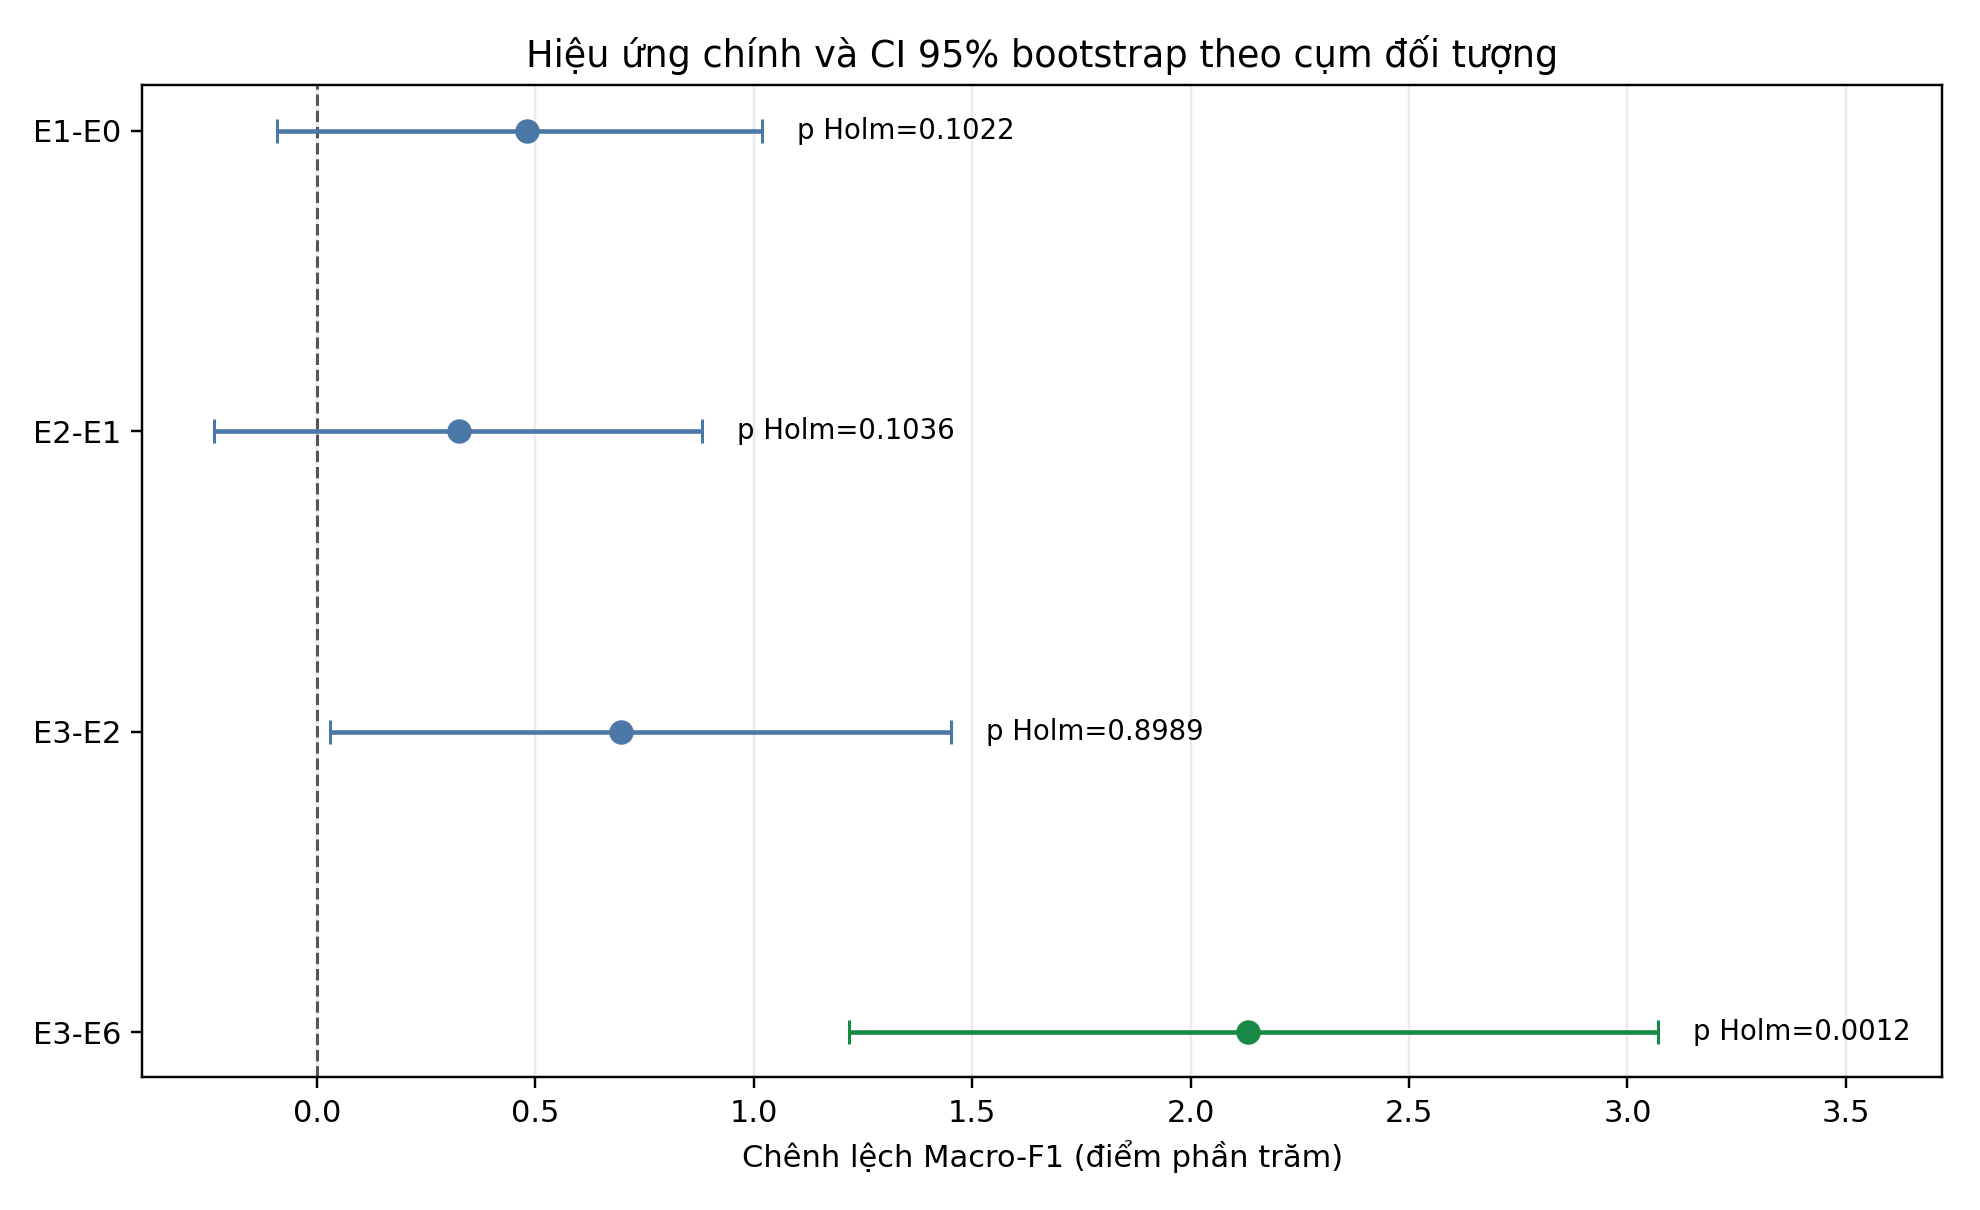
\includegraphics[width=\textwidth]{figures/gate8_primary_effects.png}
\caption{Chênh lệch \mf\ và khoảng tin cậy bootstrap cụm theo đối tượng. Trục hoành dùng điểm phần trăm.}
\label{fig:primary_effects}
\end{figure}

E1--E0 và E2--E1 có mức tăng mô tả nhỏ, nhưng CI chứa 0 và $p$ Holm lớn hơn 0,05. Vì vậy chưa đủ bằng chứng rằng TCN tốt hơn BiLSTM hoặc ResNet-1D tốt hơn 15CNN về \mf. E3--E2 có CI gộp vừa dương nhưng chỉ 37/78 người tăng, median chênh lệch theo người âm và Wilcoxon không có ý nghĩa; lợi ích không đồng đều theo đối tượng. E3--E6 là kết quả nhất quán nhất theo cả bootstrap và Wilcoxon-Holm.

\begin{table}[H]
\centering
\caption{Đối chiếu hậu nghiệm toàn pipeline E3 với mốc E0}
\label{tab:posthoc_e3_e0}
\begin{tabular}{lrrrr}
\toprule
\textbf{So sánh} & \textbf{$\Delta$ \mf} & \textbf{CI 95\% bootstrap} & \textbf{$p$ Wilcoxon} & \textbf{Thắng/Hòa/Thua} \\
\midrule
E3--E0 & 0,015024 & $[0,005746;\ 0,025871]$ & 0,012321 & 49/0/29 \\
\bottomrule
\end{tabular}
\end{table}

Đây là phân tích \emph{hậu nghiệm}, không thuộc bốn đối chiếu xác nhận ở Bảng~\ref{tab:primary_stats}. Nếu chỉ tham khảo phép Holm khi ghép nó thành so sánh thứ năm với bốn so sánh cũ, $p$ hiệu chỉnh là 0,049282; con số này không biến giả thuyết hậu nghiệm thành giả thuyết định trước. Kết quả hỗ trợ rằng toàn bộ pipeline E3 cao hơn E0 trong chiến dịch seed 42 hiện tại. Vì E3 và E0 đồng thời khác mô hình chuỗi, bộ trích xuất và tiền xử lý, đối chiếu này không xác định thành phần nào gây ra chênh lệch, không chứng minh ưu thế trên quần thể khác và không phải kiểm định tương đương hoặc không thua kém.

Chênh lệch F1 E3--E6 theo lớp lần lượt là W $+0,00255$, N1 $+0,01520$, N2 $+0,01295$, N3 $+0,06278$ và REM $+0,01311$. E4--E2, phân tích thứ cấp riêng lọc dải, có $\Delta=0,005586$, CI $[-0,001699;0,013618]$, $p=0,902877$ và thắng/thua 38/40; chưa có bằng chứng về cải thiện đồng đều.

\subsection{Gate 6: độ phức tạp và tốc độ}

\begin{table}[H]
\centering
\caption{Benchmark forward trên Tesla V100, 100 epoch mỗi lượt}
\label{tab:complexity}
\resizebox{\textwidth}{!}{%
\begin{tabular}{lrrrrrr}
\toprule
\textbf{E} & \textbf{Tham số} & \textbf{Độ trễ trung vị (ms)} & \textbf{p95 (ms)} & \textbf{Epoch/s} & \textbf{Peak MiB} & \textbf{Nhanh hơn E0} \\
\midrule
E0 & 248.630 & 13,4315 & 15,4400 & 7.445 & 58,81 & 1,00$\times$ \\
E1 & 640.950 & 12,5111 & 13,6892 & 7.993 & 60,31 & 1,07$\times$ \\
E2 & 1.085.578 & 3,5750 & 3,6531 & 27.972 & 75,54 & 3,76$\times$ \\
E3 & 1.085.578 & 3,5687 & 3,6813 & 28.021 & 75,54 & 3,76$\times$ \\
E4 & 1.085.578 & 3,5739 & 3,6427 & 27.980 & 75,54 & 3,76$\times$ \\
E6 & 1.085.578 & 3,5756 & 3,6426 & 27.967 & 75,54 & 3,76$\times$ \\
\bottomrule
\end{tabular}}
\end{table}

\begin{figure}[H]
\centering
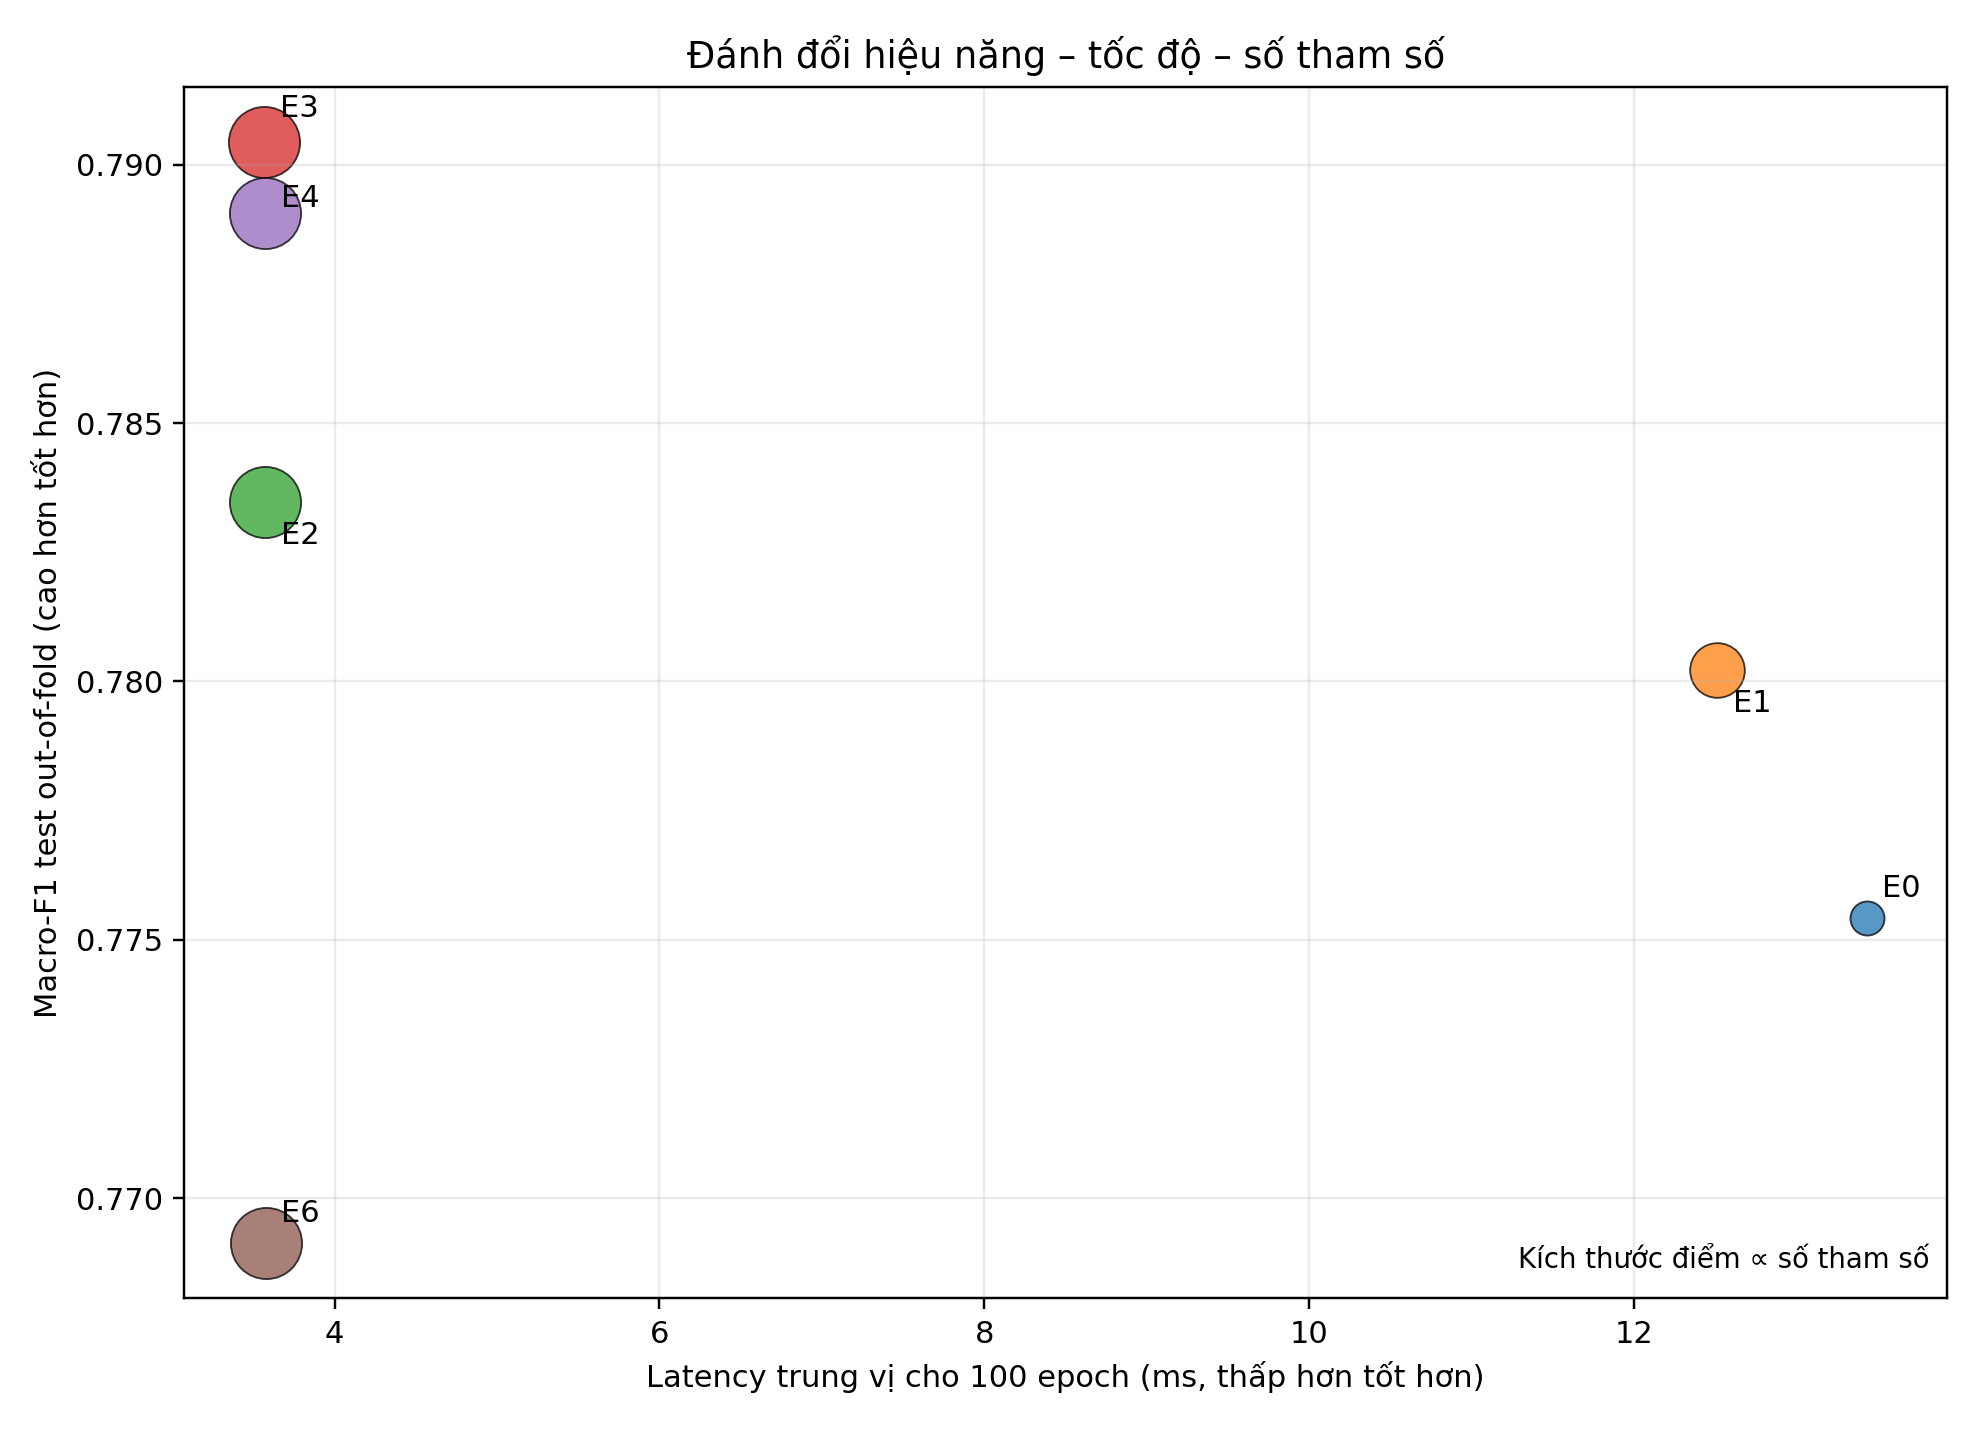
\includegraphics[width=0.9\textwidth]{figures/gate8_performance_speed_tradeoff.png}
\caption{Đánh đổi giữa \mf, độ trễ và số tham số. Diện tích điểm tỷ lệ với số tham số.}
\label{fig:tradeoff}
\end{figure}

ResNet-1D--TCN giảm từ 16 xuống 2 mô hình thành phần và nhanh hơn E0 khoảng 3,76 lần. Đổi lại, số tham số tăng 4,37 lần và peak VRAM tăng 28,4\%. Vì vậy kết quả hỗ trợ ``gọn hơn về vận hành'', không hỗ trợ ``mô hình nhẹ'' hoặc ``tiết kiệm tham số''.

\subsection{Gate 6: không gian đặc trưng}

Silhouette E2 thấp hơn E1 trong 10/10 fold. Chênh lệch E2--E1 trung bình là $-0,107851$, trung vị $-0,110025$ và khoảng quan sát $[-0,152622;-0,060811]$.

\begin{figure}[H]
\centering
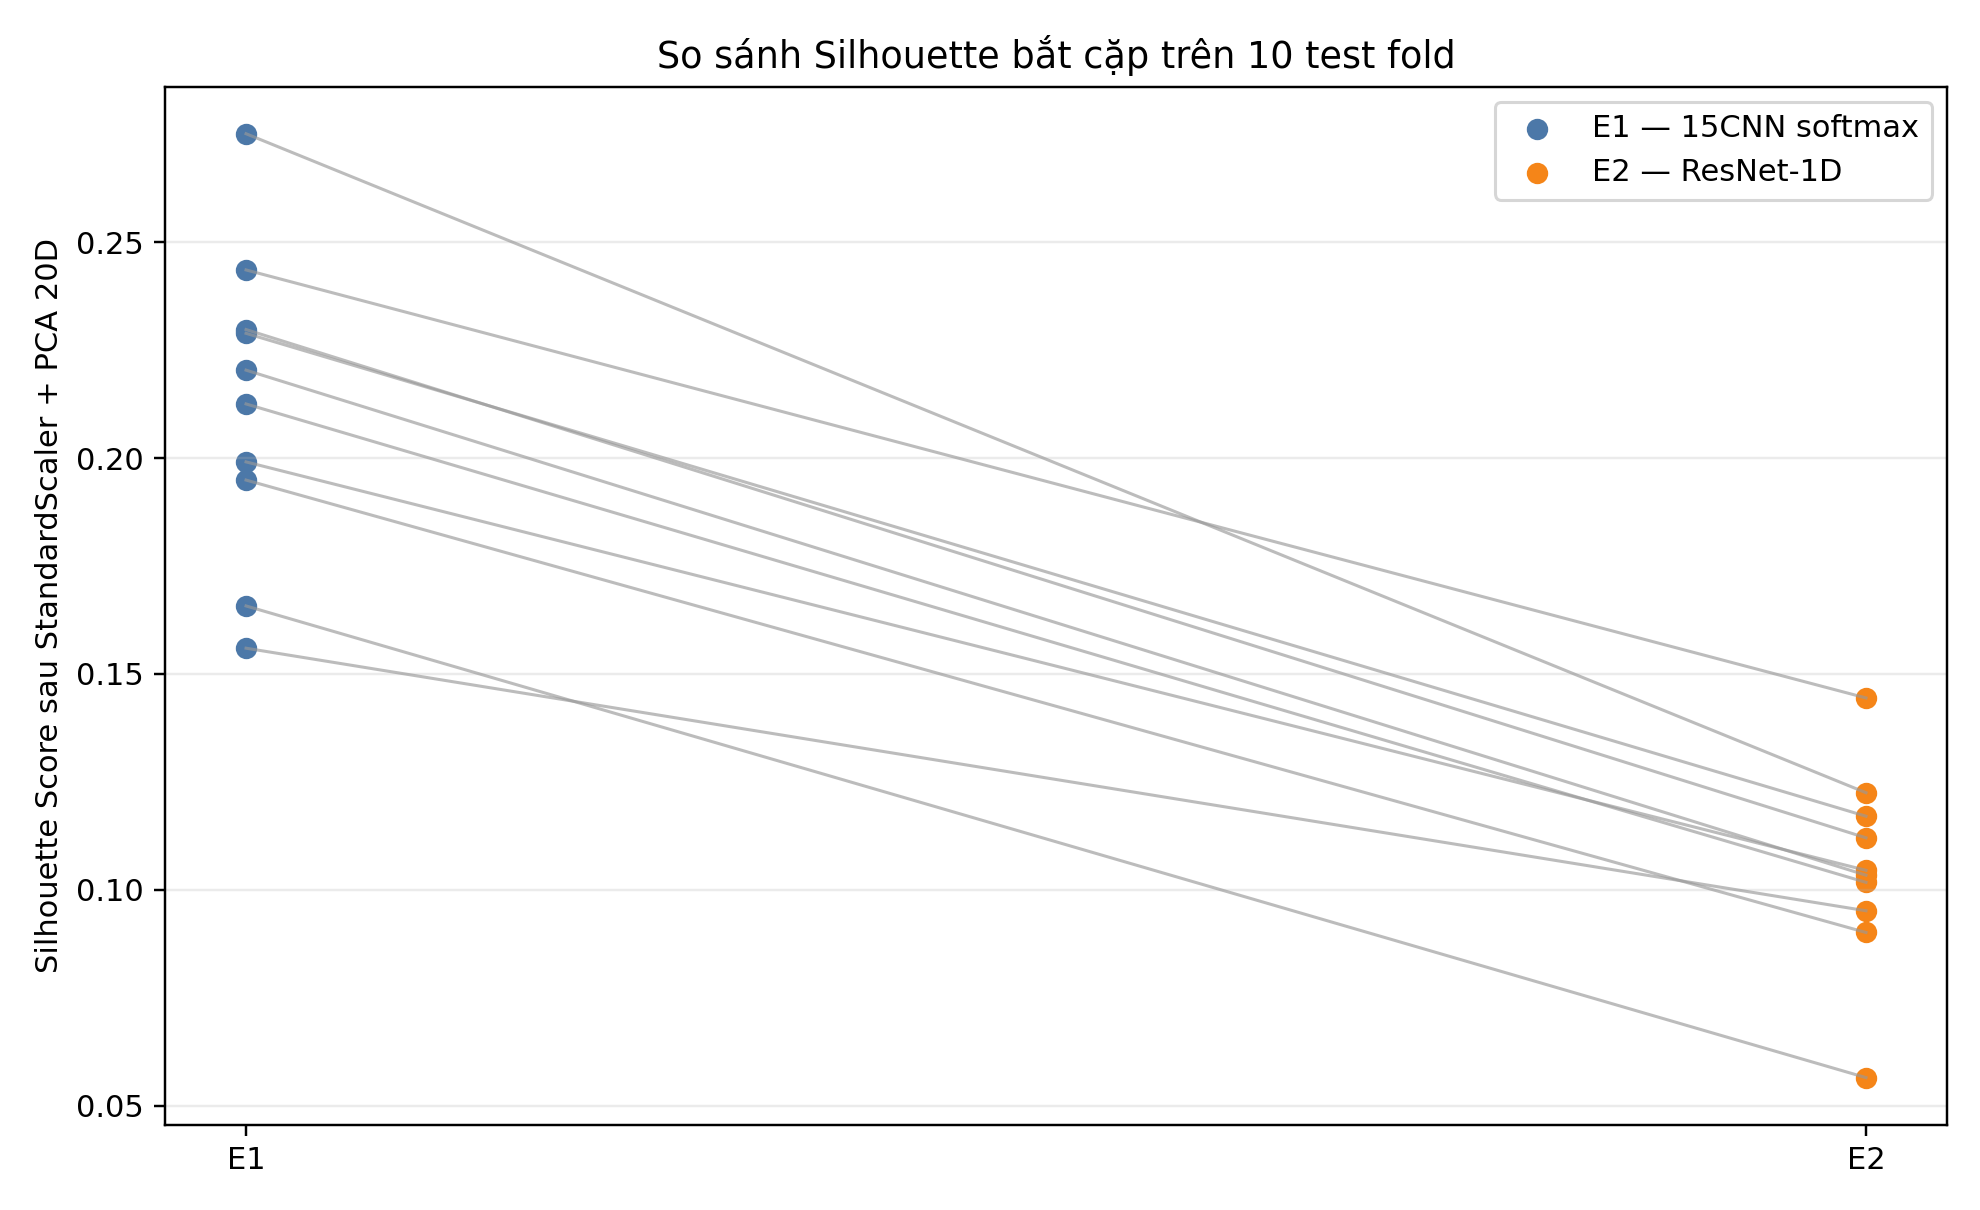
\includegraphics[width=\textwidth]{figures/gate8_feature_silhouette.png}
\caption{Silhouette bắt cặp E1/E2 sau StandardScaler và PCA 20 chiều.}
\label{fig:silhouette}
\end{figure}

Phép đo này không hỗ trợ giả thuyết rằng embedding ResNet có cụm Euclid tách biệt hơn softmax 15CNN. Nó cũng không chứng minh 15CNN tốt hơn cho dự đoán chuỗi, vì TCN có thể khai thác thông tin không biểu hiện dưới dạng cụm compact.

\subsection{Gate 7: gói công bố và truy nguyên}

Gate 7 không huấn luyện hoặc mở lại test. Cổng này sinh bảng CSV, hình, bản thảo tiếng Việt, ma trận tuyên bố--bằng chứng, manifest SHA-256 và trình kiểm định độc lập từ artifact Gate 5--6. Việc tách dữ liệu máy đọc khỏi văn bản giúp ngăn chép sai số và cho phép xây lại gói công bố.

\subsection{Gate 8: ablation nhóm C/P/N}

Gate 8 hoàn tất 30/30 lần huấn luyện validation và 30/30 lần suy luận test cho C, CP và CN; Full CPN tái sử dụng E1. Mỗi điều kiện phủ 78 đối tượng, 153 bản ghi và 195.469 epoch hợp lệ.

\begin{table}[H]
\centering
\caption{Kết quả mô tả ablation C/P/N}
\label{tab:gate8_descriptive}
\resizebox{\textwidth}{!}{%
\begin{tabular}{lrrrrr}
\toprule
\textbf{Điều kiện} & \textbf{\mf\ toàn bộ} & \textbf{F1 N1} & \textbf{Recall N1} & \textbf{\mf\ chuyển pha} & \textbf{Recall N1 chuyển pha} \\
\midrule
Full CPN & 0,780230 & 0,511469 & 0,503531 & 0,620055 & 0,483989 \\
C & 0,777477 & 0,501071 & 0,499907 & 0,619102 & 0,480828 \\
CP & 0,777733 & 0,502185 & 0,499257 & 0,617686 & 0,480163 \\
CN & 0,781585 & 0,505505 & 0,493867 & 0,618895 & 0,472428 \\
\bottomrule
\end{tabular}}
\end{table}

\begin{table}[H]
\centering
\caption{So sánh chính tại vùng chuyển pha $\pm1$ epoch}
\label{tab:gate8_stats}
\begin{tabular}{lrrrl}
\toprule
\textbf{So sánh} & \textbf{$\Delta$ \mf} & \textbf{CI 95\%} & \textbf{$p$ Holm} & \textbf{Thắng/Hòa/Thua} \\
\midrule
Full CPN--C & 0,000953 & $[-0,004588;0,006568]$ & 1,000 & 36/0/42 \\
Full CPN--CP & 0,002369 & $[-0,002990;0,007714]$ & 1,000 & 41/0/37 \\
Full CPN--CN & 0,001160 & $[-0,003918;0,006490]$ & 1,000 & 38/0/40 \\
\bottomrule
\end{tabular}
\end{table}

\begin{figure}[H]
\centering
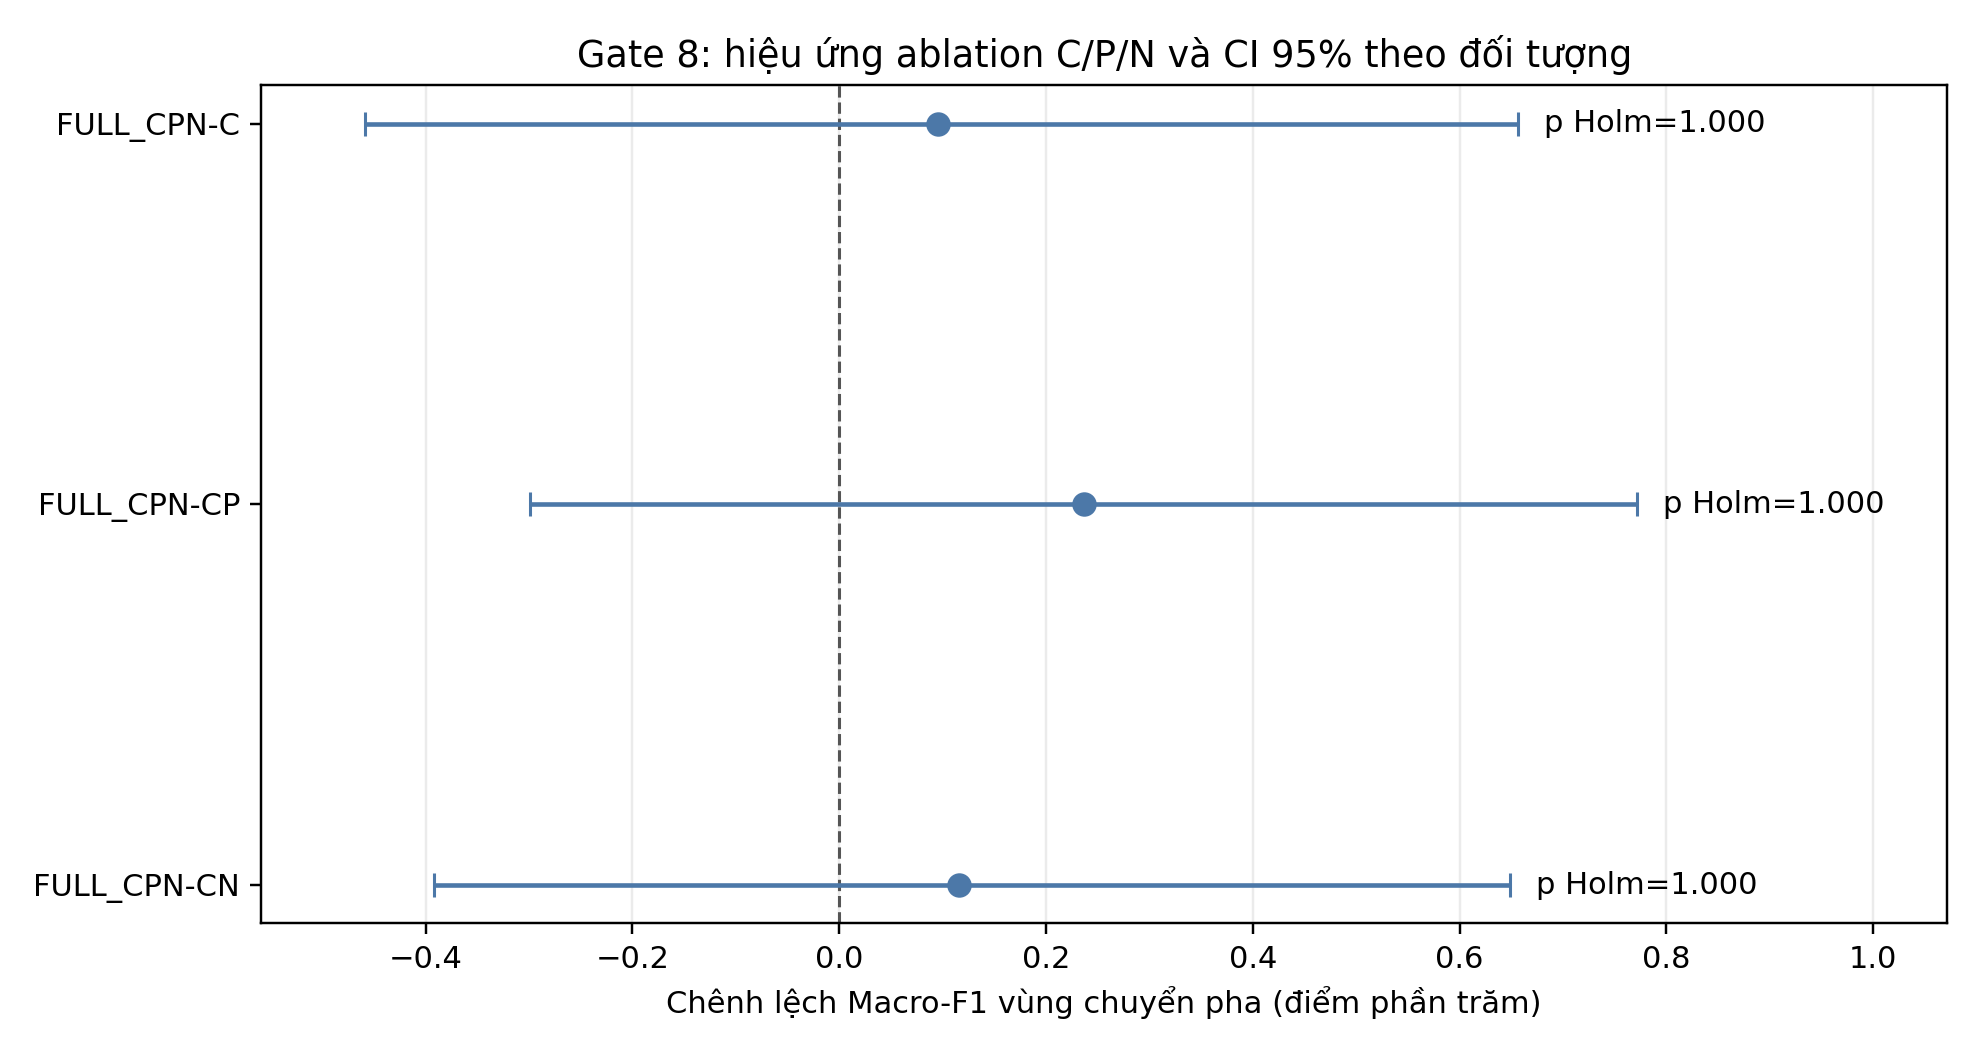
\includegraphics[width=\textwidth]{figures/gate8_context_ablation_effects.png}
\caption{Hiệu ứng ablation C/P/N tại vùng chuyển pha và CI bootstrap theo đối tượng.}
\label{fig:gate8_effects}
\end{figure}

Cả ba CI chứa 0, $p$ Holm đều bằng 1 và số người thắng/thua không nhất quán. Do đó chưa quan sát thấy lợi ích tăng thêm có ý nghĩa của P/N cho \mf\ vùng chuyển pha trong thiết kế hiện tại. Kết quả không chứng minh P/N vô dụng, không đo phần trăm thông tin và không thiết lập tương đương giữa các điều kiện.

\subsection{Chiến dịch SHHS1 zero-shot}

Tiền xử lý và hai cổng suy luận SHHS được thực hiện sau khi Gate 8 đã đóng. Validation gồm 15 đối tượng, 450 dự đoán theo fold và 45 tổ hợp; test gồm 180 đối tượng, 5.400 dự đoán theo fold và 540 tổ hợp. Hai cổng độc lập đều trả \code{PASSED} với 0 lỗi. Test có 169.012 epoch hợp lệ và mất 6.692,6 giây trên CPU 12 luồng.

\begin{table}[H]
\centering
\caption{Hiệu năng zero-shot trên 180 đối tượng SHHS1 đã khóa}
\label{tab:shhs_descriptive}
\resizebox{\textwidth}{!}{%
\begin{tabular}{lrrrrrr}
\toprule
\textbf{E} & \textbf{\mf\ đối tượng} & \textbf{CI 95\%} & \textbf{\mf\ gộp} & \textbf{Accuracy} & \textbf{$\kappa$} & \textbf{F1 N1} \\
\midrule
E0 & 0,5268 & $[0,5101;0,5431]$ & 0,5761 & 0,6648 & 0,5339 & 0,2998 \\
E3 & \textbf{0,5680} & $\mathbf{[0,5503;0,5850]}$ & \textbf{0,6099} & \textbf{0,7016} & \textbf{0,5801} & \textbf{0,3451} \\
E6 & 0,5407 & $[0,5227;0,5584]$ & 0,5732 & 0,6742 & 0,5408 & 0,3102 \\
\bottomrule
\end{tabular}}
\end{table}

\mf\ đối tượng là trung bình của 180 \mf\ tính riêng từng người và là tiêu chí chính. \mf\ gộp cho trọng số lớn hơn đối tượng có nhiều epoch nên chỉ là mô tả thứ cấp. E3 có giá trị cao nhất theo cả hai cách tổng hợp, accuracy, $\kappa$ và F1 N1.

\begin{table}[H]
\centering
\caption{Hai so sánh zero-shot chính bắt cặp theo đối tượng}
\label{tab:shhs_primary}
\resizebox{\textwidth}{!}{%
\begin{tabular}{lrrrrr}
\toprule
\textbf{So sánh} & \textbf{$\Delta$ \mf\ đối tượng} & \textbf{CI 95\%} & \textbf{Trung vị $\Delta$} & \textbf{Thắng/Hòa/Thua} & \textbf{$p$ Holm} \\
\midrule
E3--E0 & \textbf{0,0412} & $\mathbf{[0,0314;0,0512]}$ & 0,0372 & 138/0/42 & $2,65\times10^{-13}$ \\
E3--E6 & \textbf{0,0274} & $\mathbf{[0,0182;0,0370]}$ & 0,0292 & 125/0/55 & $1,87\times10^{-8}$ \\
\bottomrule
\end{tabular}}
\end{table}

\begin{figure}[H]
\centering
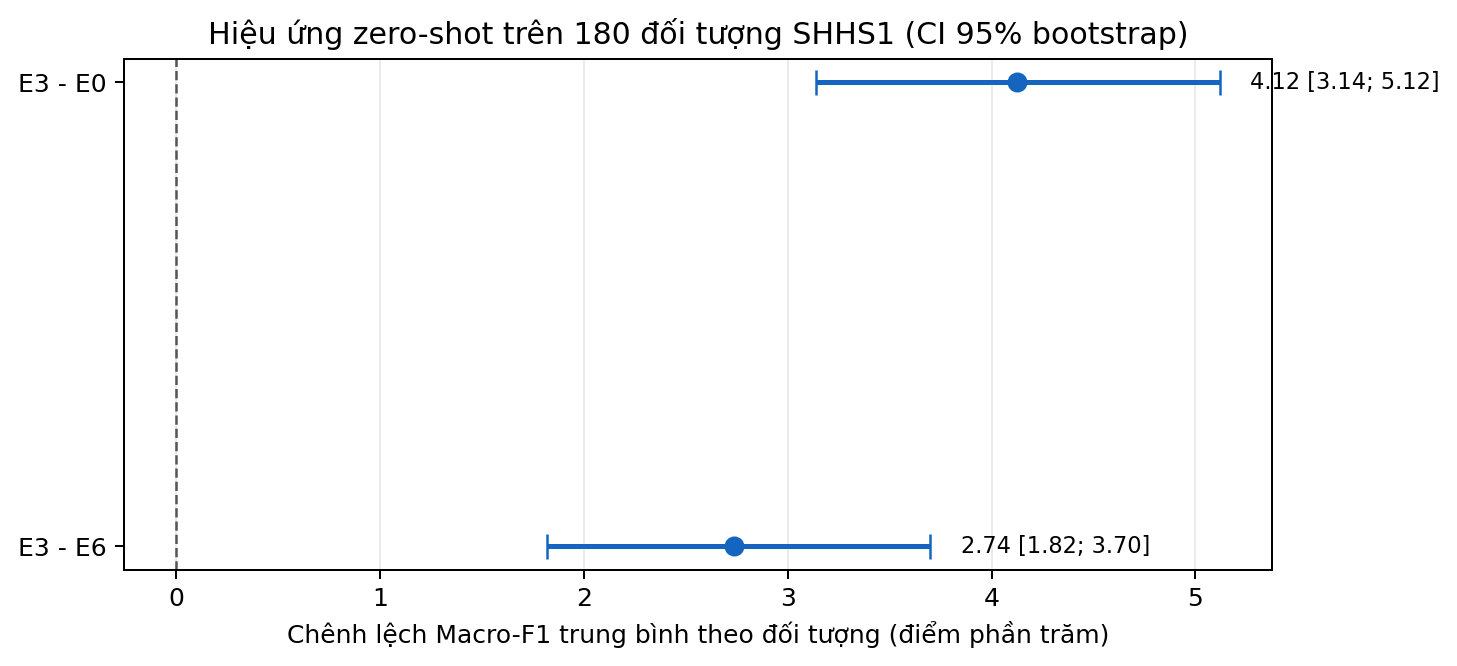
\includegraphics[width=0.92\textwidth]{figures/shhs_zero_shot_effects.png}
\caption{Chênh lệch \mf\ trung bình theo đối tượng và CI 95\% bootstrap cụm trên mẫu SHHS1. Đơn vị trục hoành là điểm phần trăm.}
\label{fig:shhs_effects}
\end{figure}

Cả hai CI chính hoàn toàn dương và Wilcoxon vẫn có ý nghĩa sau Holm. Do đó E3 có \mf\ trung bình theo đối tượng cao hơn E0 và E6 trong mẫu SHHS1 và giao thức zero-shot đã khóa. Các chỉ số hỗ trợ nhất quán: E3--E0 tăng \mf\ gộp 0,0338, accuracy 0,0368 và $\kappa$ 0,0461; E3--E6 tăng lần lượt 0,0367, 0,0274 và 0,0392. Tại 44.744 epoch nằm trong $\pm1$ epoch quanh chuyển pha thật liên tiếp, E3 tăng \mf\ so với E0 0,0366, CI $[0,0262;0,0471]$, và so với E6 0,0183, CI $[0,0092;0,0268]$.

N1 vẫn là lớp khó nhất. E3 có F1 N1 cao hơn E0/E6, nhưng recall N1 của E0 là 0,5841, cao hơn E3 0,5437; precision N1 của E3 là 0,2528, cao hơn E0 0,2017. Vì vậy lợi ích F1 của E3 phản ánh cân bằng precision--recall tốt hơn, không phải tăng đồng thời mọi chỉ số N1.

\subsection{Phân tích bổ sung thành phần E1/E2 trên SHHS1}

Sau chiến dịch zero-shot v1, một giao thức riêng được khóa trước lần suy luận SHHS đầu tiên của E1/E2. E0 được tái sử dụng nguyên trạng từ v1; E1 và E2 cùng dùng \code{paper\_raw\_v1}, đủ 10 checkpoint theo fold và không cập nhật trọng số bằng SHHS. Validation kỹ thuật gồm 300 dự đoán fold và 30 ensemble; test gồm 3.600 dự đoán fold và 360 ensemble. Hai cổng đều \code{PASSED} với 0 lỗi. Test dùng 180 đối tượng, 169.012 epoch và mất 5.681,1 giây trên CPU 12 luồng.

\begin{table}[H]
\centering
\caption{Hiệu năng mô tả trong phân tích thành phần SHHS1}
\label{tab:shhs_component_descriptive}
\resizebox{\textwidth}{!}{%
\begin{tabular}{lrrrrrr}
\toprule
\textbf{E} & \textbf{\mf\ đối tượng} & \textbf{\mf\ gộp} & \textbf{Accuracy} & \textbf{$\kappa$} & \textbf{F1 N1} & \textbf{\mf\ chuyển pha} \\
\midrule
E0 & 0,5268 & 0,5761 & 0,6648 & 0,5339 & 0,2998 & 0,4323 \\
E1 & \textbf{0,5333} & \textbf{0,5822} & \textbf{0,6709} & \textbf{0,5409} & \textbf{0,3197} & \textbf{0,4352} \\
E2 & 0,5205 & 0,5668 & 0,6656 & 0,5327 & 0,2833 & 0,4219 \\
\bottomrule
\end{tabular}}
\end{table}

\begin{table}[H]
\centering
\caption{So sánh bắt cặp trong phân tích thành phần SHHS1}
\label{tab:shhs_component_comparisons}
\resizebox{\textwidth}{!}{%
\begin{tabular}{lrrrrrl}
\toprule
\textbf{So sánh} & \textbf{$\Delta$ \mf\ đối tượng} & \textbf{CI 95\%} & \textbf{Trung vị $\Delta$} & \textbf{Thắng/Hòa/Thua} & \textbf{$p$ Holm} & \textbf{Quy tắc khóa trước} \\
\midrule
E1--E0 & \textbf{0,00651} & $\mathbf{[0,00192;0,01087]}$ & 0,00648 & 108/0/72 & 0,00325 & Đạt \\
E2--E1 & \textbf{$-0,01280$} & $\mathbf{[-0,02209;-0,00350]}$ & $-0,00429$ & 80/0/100 & 0,01005 & Không đạt \\
\bottomrule
\end{tabular}}
\end{table}

E1--E0 thỏa đồng thời điều kiện CI chính hoàn toàn dương và Wilcoxon có ý nghĩa sau Holm. Hiệu ứng nhỏ và lợi ích tại vùng chuyển pha chưa chắc chắn: $\Delta=0,00288$, CI $[-0,00297;0,00850]$. Giả thuyết E2 cao hơn E1 không đạt; chênh lệch quan sát có hướng ngược lại và cũng âm ở \mf\ gộp lẫn vùng chuyển pha. Vì 180 đối tượng này đã được mở trước cho E0/E3/E6, phân tích được mô tả là bằng chứng ngoại miền thứ cấp khóa trước suy luận E1/E2, không phải tái lập độc lập trên cohort chưa mở.

\subsection{Đối chiếu hậu nghiệm E3--E2 trên SHHS1}

E2 và E3 cùng dùng ResNet-1D--TCN nhưng khác chế độ dữ liệu: E2 dùng \code{paper\_raw\_v1}, còn E3 dùng \code{filtered\_v2}. Mọi dự đoán được ghép đúng 180 đối tượng và 169.012 epoch trước khi tính hiệu ứng.

\begin{table}[H]
\centering
\caption{Phân tích bắt cặp hậu nghiệm E3--E2 trên SHHS1}
\label{tab:shhs_e3_e2}
\resizebox{\textwidth}{!}{%
\begin{tabular}{lrrr}
\toprule
\textbf{Chỉ số E3--E2} & \textbf{Chênh lệch} & \textbf{CI 95\%} & \textbf{Ghi chú} \\
\midrule
\mf\ trung bình theo đối tượng & \textbf{0,04750} & $\mathbf{[0,03724;0,05792]}$ & Wilcoxon $p=2,35\times10^{-17}$ \\
\mf\ gộp & 0,04304 & $[0,03249;0,05364]$ & 169.012 epoch \\
Accuracy & 0,03599 & $[0,02542;0,04700]$ & Chỉ số hỗ trợ \\
$\kappa$ & 0,04737 & $[0,03382;0,06119]$ & Chỉ số hỗ trợ \\
F1 N1 & 0,06183 & $[0,03808;0,08572]$ & Chỉ số hỗ trợ \\
Recall N1 & 0,19095 & $[0,15125;0,22966]$ & Chỉ số hỗ trợ \\
\mf\ chuyển pha & 0,04700 & $[0,03790;0,05661]$ & Vùng $\pm1$ epoch \\
\bottomrule
\end{tabular}}
\end{table}

Trung vị chênh lệch \mf\ theo người là 0,04194 và E3 thắng/hòa/thua E2 trên 147/0/33 đối tượng. Tất cả CI hỗ trợ trong Bảng~\ref{tab:shhs_e3_e2} đều hoàn toàn dương. Vì vậy có bằng chứng hỗ trợ mạnh rằng toàn pipeline E3 tổng quát zero-shot tốt hơn E2 trên mẫu SHHS1 này. Trái lại, E3--E2 trên Sleep-EDF chỉ tăng \mf\ gộp 0,00696 nhưng Wilcoxon $p=0,89893$ và thắng/thua 37/41. Mẫu hình kết hợp phù hợp với cách diễn giải rằng lợi ích của chế độ tiền xử lý E3 biểu hiện rõ hơn khi chuyển miền; nó không chứng minh cơ chế nhân quả của từng thao tác tiền xử lý.

\subsection{Mở rộng đánh giá chế độ lọc dải trên SHHS với seed 123}
\label{sec:shhs_seed123_extension}

Một phân tích mở rộng được thực hiện trên cùng mẫu 180 đối tượng SHHS1 để đối chiếu trực tiếp chế độ lọc dải với các chế độ xử lý biên độ khác. Toàn bộ năm cấu hình trong phân tích này sử dụng checkpoint seed 123; không cấu hình nào được cập nhật trọng số bằng dữ liệu SHHS. Vì cohort đã được mở trong chiến dịch chính, kết quả được xem là bằng chứng bổ sung sau giao thức.

\begin{table}[H]
\centering
\caption{Kết quả mô tả của phân tích mở rộng SHHS1}
\label{tab:shhs_seed123_extension}
\resizebox{\textwidth}{!}{%
\begin{tabular}{lrrrr}
\toprule
\textbf{Cấu hình} & \textbf{\mf\ đối tượng} & \textbf{\mf\ gộp} & \textbf{Accuracy} & \textbf{$\kappa$} \\
\midrule
E0 & 0,5303 & 0,5785 & 0,6738 & 0,5420 \\
E2 & 0,5409 & 0,5858 & 0,6874 & 0,5597 \\
E3 & 0,5634 & 0,6031 & 0,7003 & 0,5772 \\
E4 & \textbf{0,5732} & \textbf{0,6147} & \textbf{0,7064} & \textbf{0,5869} \\
E6 & 0,5503 & 0,5865 & 0,6873 & 0,5552 \\
\bottomrule
\end{tabular}}
\end{table}

E4 vượt E2 0,0323 điểm Macro-F1 trung bình theo người. CI 95\% là $[0,0236;0,0410]$, Wilcoxon--Holm $p=7,40\times10^{-13}$ và thắng/hòa/thua 135/1/44. E4 cũng cao hơn E3 0,0098 điểm. Bảng~\ref{tab:shhs_seed123_pairs} trình bày đầy đủ family bốn đối chiếu của phần mở rộng, tách khỏi family hai đối chiếu SHHS chính. E4 chỉ lọc dải còn E3 thêm giới hạn/đổi thang; kết quả không tách riêng tác động của từng thao tác hoặc tương tác với huấn luyện.

\begin{table}[H]
\centering
\caption{Các đối chiếu bắt cặp SHHS1 seed 123; Holm áp dụng trong family bốn đối chiếu mở rộng}
\label{tab:shhs_seed123_pairs}
\small
\begin{tabular}{lrrr}
\toprule
\textbf{Đối chiếu} & \textbf{$\Delta$ Macro-F1 theo người} & \textbf{CI 95\%} & \textbf{$p_{Holm}$} \\
\midrule
E4--E2 & 0,0323 & $[0,0236;0,0410]$ & $7,40\times10^{-13}$ \\
E3--E4 & $-0,0098$ & $[-0,0125;-0,0073]$ & $1,89\times10^{-10}$ \\
E3--E6 & 0,0131 & $[0,0023;0,0239]$ & 0,0085 \\
E3--E0 & 0,0331 & $[0,0225;0,0438]$ & $5,19\times10^{-9}$ \\
\bottomrule
\end{tabular}
\end{table}

Trong năm cấu hình của phần mở rộng, E4 đạt F1 N1 và Macro-F1 vùng lân cận thay đổi nhãn cao nhất. Đây là bằng chứng bổ sung về ảnh hưởng của các cấu hình tiền xử lý trên cùng cohort đã mở, không phải kiểm định trực tiếp rằng tiền xử lý quan trọng hơn kiến trúc.

\section{Thảo luận}
\label{sec:discussion}

\subsection{Ba phát hiện chính}

Thứ nhất, ResNet-1D--TCN đem lại lợi ích vận hành rõ rệt mà điểm số tổng thể không phản ánh hết. Trên benchmark đã đo, thời gian suy luận giảm tương ứng mức tăng tốc 3,76 lần; chiến dịch huấn luyện và xác thực seed 123 của E3 hoàn tất trong 3 giờ 16 phút 40 giây, so với 33 giờ 35 phút 36 giây của E0. Những lợi ích này đi cùng số tham số cao hơn 4,37 lần và bộ nhớ GPU cực đại cao hơn 28,4\%. Đây là một đánh đổi có thể cân nhắc khi xây dựng pipeline, không phải sự thu nhỏ mô hình trên mọi phương diện.

Thứ hai, lợi ích dự báo phụ thuộc vào cấu hình và miền đánh giá. E1--E0 giữ encoder/đặc trưng nhưng thay cả mô hình chuỗi và lịch huấn luyện; E2--E1 thay gói đặc trưng/ngữ cảnh cùng cách huấn luyện encoder. Hai chênh lệch nhỏ trên Sleep-EDF chưa đạt ý nghĩa Wilcoxon sau Holm. Trên SHHS1, E1--E0 dương nhưng nhỏ, còn E2--E1 âm. Ngược lại, E3 vượt E0 và E6 trong hai đối chiếu SHHS chính đã khóa, đồng thời có chênh lệch gộp E3--E6 dương ở cả hai seed Sleep-EDF. Kết quả cho phép đánh giá các cấu hình đã triển khai, nhưng không tách một tác động kiến trúc thuần.

Thứ ba, lợi thế tổng thể không đồng nghĩa khắc phục được mọi lớp. E0 và E3 chỉ đạt recall N3 0,2610 và 0,2582 trên SHHS1, với hơn 72\% epoch N3 bị gán thành N2 ở cả hai mô hình. E6 còn có recall N3 thấp hơn, 0,2005. Sự tái diễn này là phát hiện trung tâm của phân tích chuyển cohort: pipeline E3 cải thiện điểm số và nhiều lớp khác, nhưng lỗi thiếu N3 vẫn tồn tại qua hai họ mô hình và không được pipeline z-score đã thử khắc phục.

\subsection{Đọc đúng các đối chiếu trong miền}

E3--E6 ở seed 42 là đối chiếu duy nhất đồng thời có CI bootstrap của chênh lệch gộp hoàn toàn dương và Wilcoxon có ý nghĩa sau Holm. Với E3--E2, CI gộp $[0,000305;0,014520]$ cũng dương, nhưng chỉ 37/78 người cải thiện và $p_{Holm}=0,8989$. Hai kết quả không mâu thuẫn: Macro-F1 từ tổng ma trận nhầm lẫn là hàm phi tuyến, còn Wilcoxon dùng các chênh lệch theo người. Chúng không thiết lập lợi ích đồng đều ở cấp đối tượng và không tự cho biết người có nhiều epoch hơn có tạo ra phần tăng gộp hay không.

Seed 123 giữ chênh lệch gộp E3--E6 dương với CI không chứa 0, nhưng không giữ ý nghĩa Wilcoxon sau Holm. Hướng hiệu ứng được lặp lại, trong khi độ lớn giảm từ 0,0213 xuống 0,0102. E4 cũng nhỉnh hơn E3 về Macro-F1 gộp ở seed 123. Vì vậy, E3 cao nhất ở chiến dịch seed 42, không phải đứng đầu mọi lần chạy; hai seed cố định chưa đủ mô tả đầy đủ biến thiên do khởi tạo.

\subsection{Lợi ích vận hành và phạm vi benchmark}

Việc giảm thời gian hoàn tất cross-validation từ hơn một ngày xuống vài giờ trên phần cứng đã đo rút ngắn vòng kiểm tra và phát triển mô hình. Tuy nhiên, wall-clock còn phụ thuộc số epoch thực chạy, optimizer, batch size, dừng sớm và việc E1 tái sử dụng encoder/cache E0. Không thể gán toàn bộ mức giảm cho phép thay BiLSTM bằng TCN. Tương tự, mức tăng tốc suy luận 3,76 lần là phép đo forward theo cửa sổ benchmark; nó không bao gồm tiền xử lý, đọc dữ liệu hoặc thời gian phải chờ ngữ cảnh tương lai. Lọc không lệch pha, BiLSTM hai chiều và TCN không nhân quả đặt hệ thống này trong bối cảnh phân tích ngoại tuyến.

\subsection{Tiền xử lý và đối chứng E6}

Trong đối chiếu hậu nghiệm SHHS1 đã quan sát, chênh lệch E3--E2 là $+0,04750$ Macro-F1 trung bình theo người, lớn hơn chênh lệch của E1--E0 và E2--E1. Phần mở rộng seed 123 cũng cho thấy E4 chỉ lọc dải cao hơn đầu vào thô E2, và cao hơn E3 cùng seed. Trong mẫu này, xử lý tín hiệu là một trục phát triển có ảnh hưởng đáng kể, không phải chi tiết triển khai trung tính. Một thiết kế nhân tố độc lập sẽ cần thiết để phân tách đóng góp của lọc dải, đổi thang và tương tác với huấn luyện.

E6 kiểm tra một lựa chọn cụ thể thường dễ áp dụng: z-score theo từng bản ghi. Trung bình và độ lệch chuẩn lấy từ toàn bộ recording đích không nhãn nên phép chuẩn hóa có tính transductive, dù trọng số vẫn chỉ học từ Sleep-EDF. Recall N3 toàn mẫu của E6 là 0,2005 so với 0,2582 của E3; tại vùng lân cận thay đổi nhãn, các giá trị là 0,0721 và 0,0733. Như vậy, pipeline z-score đã thử không khắc phục thiếu N3. Do E6 được huấn luyện riêng với đầu vào chuẩn hóa tương ứng, đây không phải can thiệp chỉ thay biên độ ở cùng một mô hình; kết quả không loại trừ vai trò của biên độ, montage hoặc hiệu quả của các phương pháp thích nghi không nhãn khác.

\subsection{Ý nghĩa của lỗi N3 và phân tích phản thực}

E3 có precision N3 0,9440 nhưng recall 0,2582: khi phát lớp N3 mô hình thường đúng, song bỏ sót phần lớn N3 thật. E0 có mẫu thiếu N3 gần tương tự. Cả hai có recall N3 thấp hơn gần thay đổi nhãn tham chiếu so với vùng ổn định, nhưng ngay trong vùng ổn định SHHS1 recall cũng chỉ là 0,4008/0,3900. Vì vậy, mô tả lỗi chỉ quanh ranh giới không bao quát toàn bộ thiếu hụt. Thành phần lớp giữa các vùng khác nhau; chênh lệch metric không xác định rằng chuyển pha sinh lý gây ra lỗi. Montage, thiết bị, quần thể và thực hành chấm cũng thay đổi đồng thời giữa hai dataset, nên chưa thể quy lỗi cho một yếu tố riêng.

Oracle sửa riêng N3$\rightarrow$N2 trong ma trận E3 nâng Macro-F1 SHHS1 từ 0,6099 lên 0,7444, tương ứng 74,5\% chênh lệch điểm quan sát với Sleep-EDF. Đây là cách định lượng quy mô kênh lỗi, không phải hiệu năng một phương pháp sẵn có hoặc phần mất mát nhân quả do dịch chuyển miền. Sleep-EDF dùng dự đoán ngoài fold, còn SHHS dùng ensemble mười mô hình; phân bố lớp và thành phần cohort cũng khác. N3$\rightarrow$N2, tiếp theo là N2$\rightarrow$REM trong E3, là các mục tiêu hợp lý cho một nghiên cứu khắc phục có kiểm chứng, nhưng oracle chưa chứng minh chiến lược thu nhãn nào tối ưu.

\subsection{Vai trò của ngữ cảnh và không gian đặc trưng}

Gate 8 chưa phát hiện lợi ích tăng thêm có ý nghĩa của các nhóm P/N được mã hóa riêng trong các điều kiện huấn luyện lại TCN. Kết quả không thiết lập tương đương hay phủ định giá trị của ngữ cảnh thời gian nói chung. Silhouette E2 thấp hơn E1 ở cả mười fold cũng chỉ mô tả cấu trúc cụm theo khoảng cách Euclid sau pipeline phân tích; không đủ xếp hạng khả năng dự đoán chuỗi của hai biểu diễn. Các phân tích này giúp giới hạn những cách giải thích về biểu diễn và ngữ cảnh, không thay thế bằng chứng hiệu năng bắt cặp.

\subsection{Giới hạn và nghiên cứu tiếp theo}

Nghiên cứu chỉ khảo sát một hướng chuyển Sleep-EDF sang mẫu 180 người SHHS1, hai seed cố định và các cấu hình cụ thể. Một số đối chiếu thành phần, phần mở rộng E4 và vùng nhãn là hậu nghiệm trên cohort đã xem kết quả. Cùng subject splits bảo vệ tính bắt cặp nhưng không biến các training recipe khác nhau thành đối chứng kiến trúc thuần. Các số liệu này hỗ trợ nghiên cứu thực nghiệm về pipeline và lỗi chuyển cohort, chưa xác nhận hiệu quả lâm sàng.

Bước kiểm chứng phù hợp có thể là lặp lại mẫu lỗi trên một cohort chưa được xem hoặc trên một pipeline đối chứng mạnh dưới cùng giao thức. Nếu mục tiêu chuyển sang khắc phục N3, có thể đánh giá calibration hoặc fine-tuning trên tập thích nghi/validation riêng, báo cáo đồng thời recall, precision và false-positive N3, ảnh hưởng lên N2, cùng kết quả tại vùng lân cận và vùng ổn định. Không dùng 180 test subjects để chọn threshold hoặc cập nhật mô hình. Nghiên cứu hiện tại chưa so sánh chi phí thu nhãn hay hiệu quả của các hướng này, nên không xếp chúng thành một thứ tự tối ưu về công sức.

\subsection{Diễn giải phân tích mở rộng E4 trên SHHS}

Trên cùng mẫu SHHS1 và cùng seed 123, E4 có \mf\ trung bình theo đối tượng cao nhất trong năm cấu hình, vượt E2 0,0323 điểm và E3 0,0098 điểm. Cấu hình chỉ lọc dải vì vậy là một đối chứng thực dụng đáng giữ khi kiểm chứng tiếp, thay vì mặc định các thao tác giới hạn/đổi thang bổ sung luôn có lợi. Đối chiếu không tách riêng tác động của từng thao tác hoặc tương tác với huấn luyện.

Phần mở rộng không thay thế hai đối chiếu SHHS chính đã khóa: cohort đã được xem kết quả và E4 chỉ được đánh giá ở seed 123 trong phần này. Xác nhận thứ hạng trên mẫu chưa xem sẽ giúp đánh giá khả năng khái quát; chưa có căn cứ xếp bước đó cao hơn mọi hướng khác theo chi phí hay công sức.

\section{Kết luận}
\label{sec:conclusion}

Nghiên cứu cung cấp một đánh giá bắt cặp về các cấu hình phân giai đoạn giấc ngủ từ EEG đơn kênh, kết nối hiệu năng trong miền, chi phí vận hành và cấu trúc lỗi ngoài miền. Trên Sleep-EDF seed 42, E3 đạt Macro-F1 ngoài fold 0,7904, cao nhất trong sáu cấu hình, và vượt E6 0,0213 với CI hoàn toàn dương cùng ý nghĩa Wilcoxon sau Holm. Seed 123 giữ hướng chênh lệch gộp E3--E6 nhưng không giữ ý nghĩa sau Holm; E4 nhỉnh hơn E3 ở lần chạy này. E1--E0 thay cả cấu hình mô hình chuỗi và lịch huấn luyện, còn E2--E1 thay gói đặc trưng/ngữ cảnh cùng cách huấn luyện encoder, nên kết quả không xác lập ưu thế kiến trúc riêng lẻ.

ResNet-1D--TCN đem lại một đánh đổi vận hành đáng kể: suy luận nhanh hơn E0 khoảng 3,76 lần trên benchmark, với số tham số cao hơn 4,37 lần và bộ nhớ GPU cực đại cao hơn 28,4\%. Trong chiến dịch seed 123, thời gian huấn luyện và xác thực 10 fold giảm từ 33 giờ 35 phút 36 giây của E0 xuống 2 giờ 44 phút 57 giây với E2 hoặc 3 giờ 16 phút 40 giây với E3. Đây là lợi ích của các cấu hình và lịch chạy đã đo, không phải tốc độ độc lập phần cứng hay độ trễ quyết định trực tuyến.

Trên 180 người SHHS1, E3 vượt E0 và E6 theo Macro-F1 trung bình ở cấp đối tượng trong hai đối chiếu đã khóa. Tuy nhiên, E0/E3 đều gán hơn 72\% N3 thành N2 và có recall N3 chỉ 0,2610/0,2582. E6 dùng thống kê toàn bản ghi đích không nhãn, có tính transductive, cũng không khắc phục thiếu N3. Sự tái diễn của lỗi qua hai họ mô hình, kể cả ở vùng nhãn ổn định, cho thấy cải thiện tổng thể và khắc phục lỗi theo lớp là hai kết quả cần được báo cáo tách biệt.

Đối chiếu hậu nghiệm E3--E2 và phần mở rộng E4 làm nổi bật ảnh hưởng của các cấu hình tiền xử lý trong mẫu đã khảo sát. Oracle N3$\rightarrow$N2 trên E3 tương ứng 74,5\% chênh lệch điểm mô tả giữa EDF ngoài fold và SHHS ensemble, chỉ ra quy mô của một kênh lỗi đáng kiểm chứng tiếp. Các bằng chứng này củng cố định vị của công trình như một nghiên cứu pipeline và chẩn đoán chuyển cohort có truy nguyên; chúng chưa xác định cơ chế sinh lý, hiệu quả thích nghi hoặc một chiến lược thu nhãn tối ưu.

\subsection{Kết luận bổ sung từ phân tích E4}

Trên cùng 180 đối tượng SHHS1 và seed 123, E4 đạt \mf\ trung bình theo đối tượng 0,5732, cao hơn E2 0,0323 điểm với CI 95\% $[0,0236;0,0410]$, đồng thời cao hơn E3 0,0098 điểm. Phần mở rộng xác định cấu hình chỉ lọc dải là một đối chứng đáng kiểm chứng tiếp; nó không thiết lập nhân quả, tương đương hay không thua kém và không thay thế hai đối chiếu SHHS chính đã khóa.

\section{Hồ sơ tái lập và truy nguyên}
\label{sec:reproducibility}

\subsection{Nguồn bằng chứng}

Các kết quả được tổng hợp từ bốn nhóm bằng chứng: dữ liệu và phép chia đã kiểm định; artifact huấn luyện/dự đoán; báo cáo thống kê bắt cặp; và gói công bố gồm bảng, hình cùng ma trận bằng chứng. Vai trò của truy nguyên là bảo đảm mỗi con số và kết luận có thể quay lại đúng artifact, không phải làm tăng điểm số hay thay thế xác nhận trên mẫu độc lập.

\begin{table}[H]
\centering
\caption{Các nhóm bằng chứng được sử dụng trong báo cáo}
\label{tab:reproducibility_evidence}
\begin{tabularx}{\textwidth}{lY}
\toprule
\textbf{Nhóm} & \textbf{Vai trò} \\
\midrule
Dữ liệu và phép chia & Xác nhận đối tượng, bản ghi, nhãn và nguyên tắc tách mẫu \\
Kết quả huấn luyện & Xác nhận mô hình đã chọn, dự đoán, chỉ số và sự tương thích giữa cấu hình \\
Phân tích thống kê & Cung cấp chênh lệch, khoảng tin cậy và kiểm định bắt cặp \\
Gói công bố & Cung cấp bảng, hình, ma trận bằng chứng và kiểm tra toàn vẹn độc lập \\
\bottomrule
\end{tabularx}
\end{table}

\subsection{Nguyên tắc kiểm tra}

Kiểm tra tái lập được thực hiện theo ba lớp: (1) cấu trúc, độ phủ và khóa bắt cặp; (2) phiên bản, mã băm và tính đầy đủ của artifact; (3) sự khớp nhau giữa bảng/hình/tuyên bố và dữ liệu nguồn. Các phép kiểm tra chỉ đọc artifact đã khóa, không huấn luyện lại mô hình hoặc mở lại test để chọn kết quả.

Lần lặp seed 123 dùng cùng dữ liệu, phép chia và họ cấu hình. Các seed được báo cáo riêng, không gộp $p$-value và không được xem như mẫu đầy đủ của biến thiên khởi tạo. Các phân tích SHHS thành phần, E3--E2 và E4 được ghi rõ là thứ cấp hoặc hậu nghiệm trên cohort đã mở.

\subsection{Tái phân tích E6 và tình trạng provenance SHHS1}

Phân tích E6 theo lớp được tính trực tiếp từ 180 artifact dự đoán chuyển miền không cập nhật trọng số đã khóa trên ổ ngoài. Chiến dịch được đánh dấu hoàn tất, test gate đạt, toàn bộ 180 mã băm artifact E6 khớp run manifest, và ma trận nhầm lẫn tính lại theo từng bản ghi khớp giá trị trong manifest. Vì vậy, các chỉ số E6 mới trong báo cáo là phép tái phân tích mô tả của dự đoán đã tồn tại, không phải một lượt suy luận mới.

Theo hồ sơ kiểm toán đã lưu, dự đoán E6 và chỉ số tính lại đã được xác minh ở cấp artifact. Trong lượt rà soát hiện tại, run manifest gốc trên ổ ngoài vẫn truy cập được và có SHA-256 \seqsplit{f9cd5ebbd20f26b188b5dc13ac6e417ff8ef0fa8dcae78760cfcb27940bf58cf}. Protocol hash ghi trong manifest (\seqsplit{165d7cdf614ff071da7bd5ca94eb4e52dd8bee1ce5eafb712c2c8a0d0550fe93}) khớp snapshot lịch sử \texttt{configs/shhs\_zero\_shot\_v1.json}. Tệp \texttt{configs/shhs\_v1\_protocol.json} hiện có hash \seqsplit{9541e2334cdae98b5d36b95a2656993cdaaffb35a3160dad70af11d14b653fe9} vì là hồ sơ mở rộng sau chạy; không thay hash lịch sử bằng hash này. Khớp hash xác nhận danh tính tệp và liên kết artifact, không tự chứng minh đăng ký trước công khai, thời điểm khóa độc lập hoặc khả năng tái sinh toàn bộ chiến dịch. Lượt chỉnh sửa báo cáo không huấn luyện hay tạo prediction mới.

\subsection{Tình trạng dữ liệu dẫn xuất}

Snapshot dữ liệu dẫn xuất gồm 765 tệp thuộc năm biến thể tiền xử lý. Kiểm toán độc lập xác nhận 765/765 tệp khớp SHA-256 trong manifest nội dung, có metadata ZIP chuẩn hóa, đọc được và nhất quán về nhãn, vị trí thời gian, hình dạng cùng quan hệ biến đổi khoa học. Mã băm container lịch sử được bảo toàn trong trường truy nguyên riêng.

Khóa byte của snapshot bảo đảm tính toàn vẹn khi lưu trữ và trao đổi, nhưng không thay thế phép tái sinh độc lập từ EDF gốc trong môi trường phần mềm đã khóa. Gói mã nguồn đi kèm giao thức và công cụ kiểm định cho bước tái sinh đó.

\subsection{Biên diễn giải khoa học}

\begin{table}[H]
\centering
\caption{Phạm vi diễn giải của các kết quả chính}
\label{tab:claim_boundaries}
\begin{tabularx}{\textwidth}{YY}
\toprule
\textbf{Kết luận được hỗ trợ} & \textbf{Diễn giải vượt quá bằng chứng} \\
\midrule
Các phép thay cấu hình E1/E2 chưa cho ưu thế ổn định & Đã cô lập kiến trúc, hoặc ResNet-1D/TCN vượt trội phổ quát \\
ResNet-1D--TCN nhanh hơn và gọn hơn về vận hành & Mô hình nhẹ hơn về tham số hoặc bộ nhớ \\
E3 cao hơn E0/E6 trên mẫu SHHS1 đã khóa & E3 đã giải quyết dịch chuyển miền hoặc vượt SOTA \\
E3--E2/E4 cho lợi ích của cấu hình tiền xử lý trên mẫu đã khảo sát & Một thao tác riêng là nguyên nhân hoặc trục tiền xử lý luôn ưu việt \\
N3$\rightarrow$N2 tái diễn ở E0/E3 và có đòn bẩy phản thực lớn nhất trên E3 & E3 gây ra lỗi này hoặc sửa kênh này chắc chắn đạt \mf\ 0,7444 \\
E6 không sửa được lỗi N3 trong pipeline này & Biên độ tuyệt đối không liên quan đến N3 \\
Gate 8 chưa cho thấy giá trị biên của P/N & Ngữ cảnh thời gian hoàn toàn vô dụng \\
Silhouette không phù hợp để chọn encoder ở đây & Embedding CNN tốt hơn ResNet cho mọi nhiệm vụ \\
Các điều kiện chưa được kiểm định tương đương & Giá trị $p$ lớn chứng minh tương đương \\
\bottomrule
\end{tabularx}
\end{table}

\subsection{Thông tin tác giả và các xác nhận trước công bố}

Ngô Nhật Quân là tác giả đứng đầu và tác giả liên hệ, email \texttt{23521258@gm.uit.edu.vn}; Phạm Thái Sơn là đồng tác giả thứ hai. Hai tác giả đã đọc và duyệt bản cuối. Ngô Nhật Quân: Conceptualization, Methodology, Software, Data curation, Formal analysis, Investigation, Visualization, Writing -- original draft, Writing -- review and editing. Phạm Thái Sơn: Validation, Investigation, Visualization, Writing -- review and editing.

Các tác giả trân trọng cảm ơn Nguyễn Hồ Duy Trí đã hướng dẫn học thuật, định hướng đề tài nghiên cứu và góp ý xây dựng cho các phiên bản trước của bản thảo.

Tác giả xác nhận đã xin được quyền truy cập SHHS qua NSRR và xác nhận phân tích thứ cấp dữ liệu đã khử định danh không cần xét duyệt đạo đức tại đơn vị áp dụng. Nghiên cứu nhận khoảng 6.000.000 VND hỗ trợ sinh viên từ Trường Đại học Công nghệ Thông tin, Đại học Quốc gia Thành phố Hồ Chí Minh; hai tác giả tuyên bố không có xung đột lợi ích. Repository mã nguồn là \url{https://github.com/quanuiter/SleepTCN}; báo cáo không công bố dữ liệu hạn chế hoặc mã định danh SHHS.

OpenAI Codex chỉ hỗ trợ biên tập, tổ chức nội dung, kiểm tra nhất quán với code/artifact và dựng hình từ các tổng hợp số liệu đã lưu; không huấn luyện thêm mô hình hoặc tạo dữ liệu thực nghiệm. Tác giả không dùng công cụ AI nào khác, hai tác giả đã đọc và duyệt bản cuối và chịu trách nhiệm về nội dung trước công bố.


\clearpage
\bibliographystyle{ieeetr}
\bibliography{references}

\end{document}
